In this chapter, I present the theoretical background necessary to understand the modeling of globular clusters and stellar streams performed in this thesis. Much of the content draws from two comprehensive introductions to galactic dynamics: Galactic Dynamics by Binney and Tremaine, and Galaxiesbook.org by Bovy. These references provide a solid foundation for the physics and mathematical tools used throughout this work.

A common assumption in galactic dynamics is the so-called fluid limit, in which the orbit of a star is determined by the smooth gravitational potential generated by the galaxy as a whole. In this approximation, interactions between individual stars are negligible. This assumption holds well in many contexts—but not in all.

Globular clusters are a notable exception. Their relatively small number of stars makes them too “grainy” for the fluid approximation to hold, yet they contain far too many stars to be treated as simple few-body systems. This intermediate regime is the subject of the aptly named Million Body Problem, explored in detail by Heggie and Hut. Their textbook provides a thorough survey of methods to address this challenge, and their preface offers an insightful summary of the central difficulty: globular clusters inhabit an awkward middle ground where neither the fluid limit nor simplified few-body interactions apply cleanly. As a result, no analytical theory fully captures their dynamics.

While this thesis focuses primarily on stellar streams—specifically, how stars escape from globular clusters and evolve under the influence of the galactic potential—it is important to acknowledge that the internal evolution of the progenitor clusters still affects the properties of the streams. Although the internal cluster dynamics lie outside the scope of this work, they place important constraints on the interpretation of our results.

The remainder of this chapter is structured to clarify the theoretical framework supporting this thesis. I divide the discussion into three main parts:

\begin{itemize}

    \item \textbf{Explicit physics} - the physical laws and initial conditions implemented in the simulations;

    \item \textbf{Implicit physics} - the emergent behavior of these systems, the assumptions involved, and the mathematical tools used to interpret the results;

    \item \textbf{Ignored physics} - relevant aspects of the problem that are beyond the scope of this thesis, but which impact the interpretation of our results. Where appropriate, I cite works that pursue these directions and discuss how future work could incorporate them to improve upon the current modeling.

\end{itemize}




\section{The Explicit Physics}
    My simulations solve the \textit{restricted three body problem}. In essence
    \begin{figure}
        \centering
        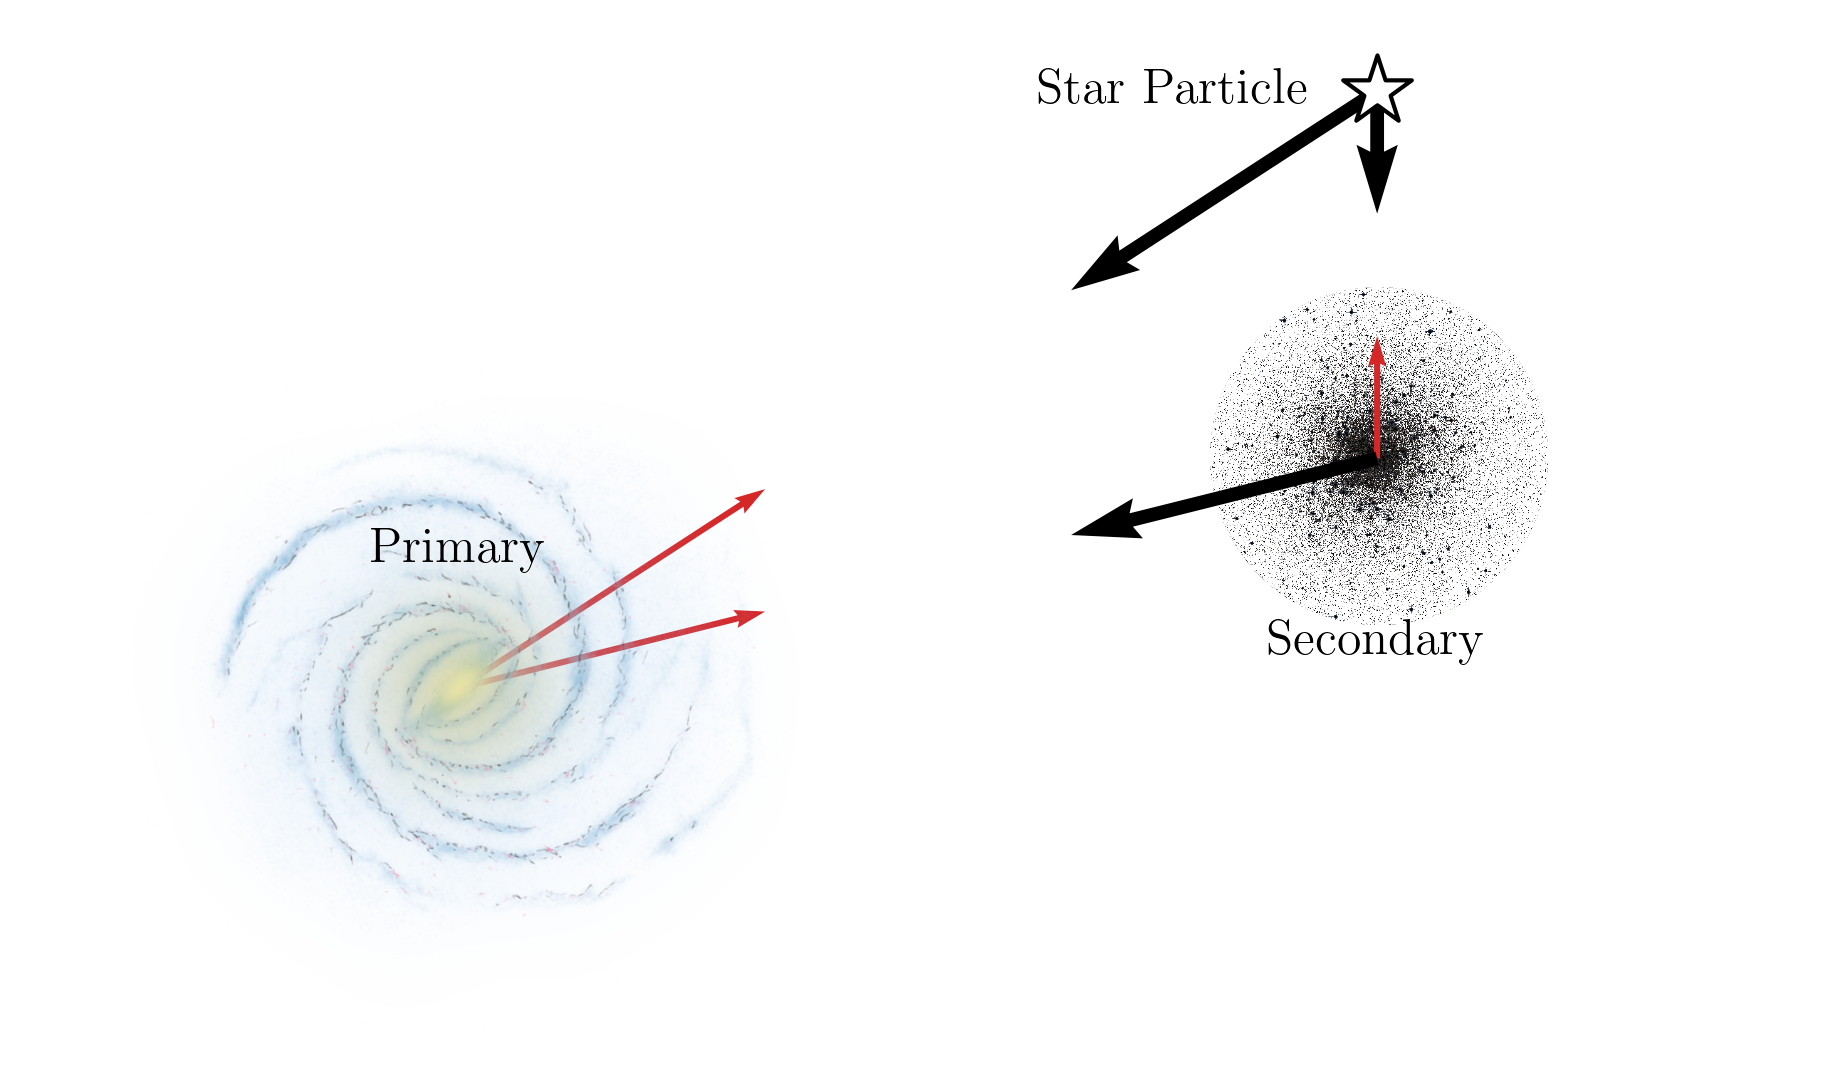
\includegraphics[width=\linewidth]{images/restricted_three_body_set_up.png}
        \caption{Little sketch of my equations of motion. }
    \end{figure}
    
    \subsection{Equations of Motion} \label{subsec:myEquationsOfMotion}
        I like to start with the \textit{Lagrangian}, which comes from the variational principle which states that particles with move along trajectories that minimize the difference, $ L = T-U $, which $L$ is the Lagrangian, $T$ is the kinetic energy and $U$ is the potential energy. Also, as is almost always the case in gravitational dynamics, we normalize by the mass and use \textit{specific} energy: 
        \begin{equation}
            \mathcal{L} = \frac{L}{m} = \frac{1}{2}\left(\dot{x}^2+\dot{y}^2+\dot{z}^2\right) - \Phi(x,y,z).
        \end{equation}
        However, Lagrange's equations give a system of three second order coupled ordinary differential equations. If we switch to Hamiltonain dynamics, we can object a set of six \textit{first} order ordinary differential equations, which is easier to implement computationally. Also, since we are using the specific energy, the momentum coordinates for Hamilton's equations are the same as the velocities from the Lagrangian: $ p_i = \frac{\partial \mathcal{L}}{\partial \dot{q}_i}$. Therefore, $p_i = \dot{q}_i$, where $i \in \left(x,y,z\right)$. The Hamilton is derived through the Legendre transform: $ \mathcal{H}=\sum_i p_i\dot{q}_i - \mathcal{L}$. Then, we can apply Hamilton's equations to obtain the set of equations: 
        \begin{align}
            \dot{p}_i &= -\frac{\partial \mathcal{H}}{\partial q_i} \\
            \dot{q}_i &= \frac{\partial \mathcal{H}}{\partial p_i}
        \end{align}

        And when written explicity become: 
        \begin{align}
            \dot{p}_x &= -\frac{\partial \Phi}{\partial x} \\
            \dot{p}_y &= -\frac{\partial \Phi}{\partial y} \\
            \dot{p}_z &= -\frac{\partial \Phi}{\partial z} \\
            \dot{x} &= p_x \\ 
            \dot{y} &= p_y \\ 
            \dot{z} &= p_z \\ 
        \end{align}        


        \subsubsection*{The Globular Cluster}
            In the case of the Globular Clusters, they only feel the Galaxy. So their Hamiltonian becomes: 
            % \begin{equation}

            % \end{equation}

        \subsubsection*{The Star Particles}

    \subsection{Potential density pairs}

        \begin{figure}
            \centering
            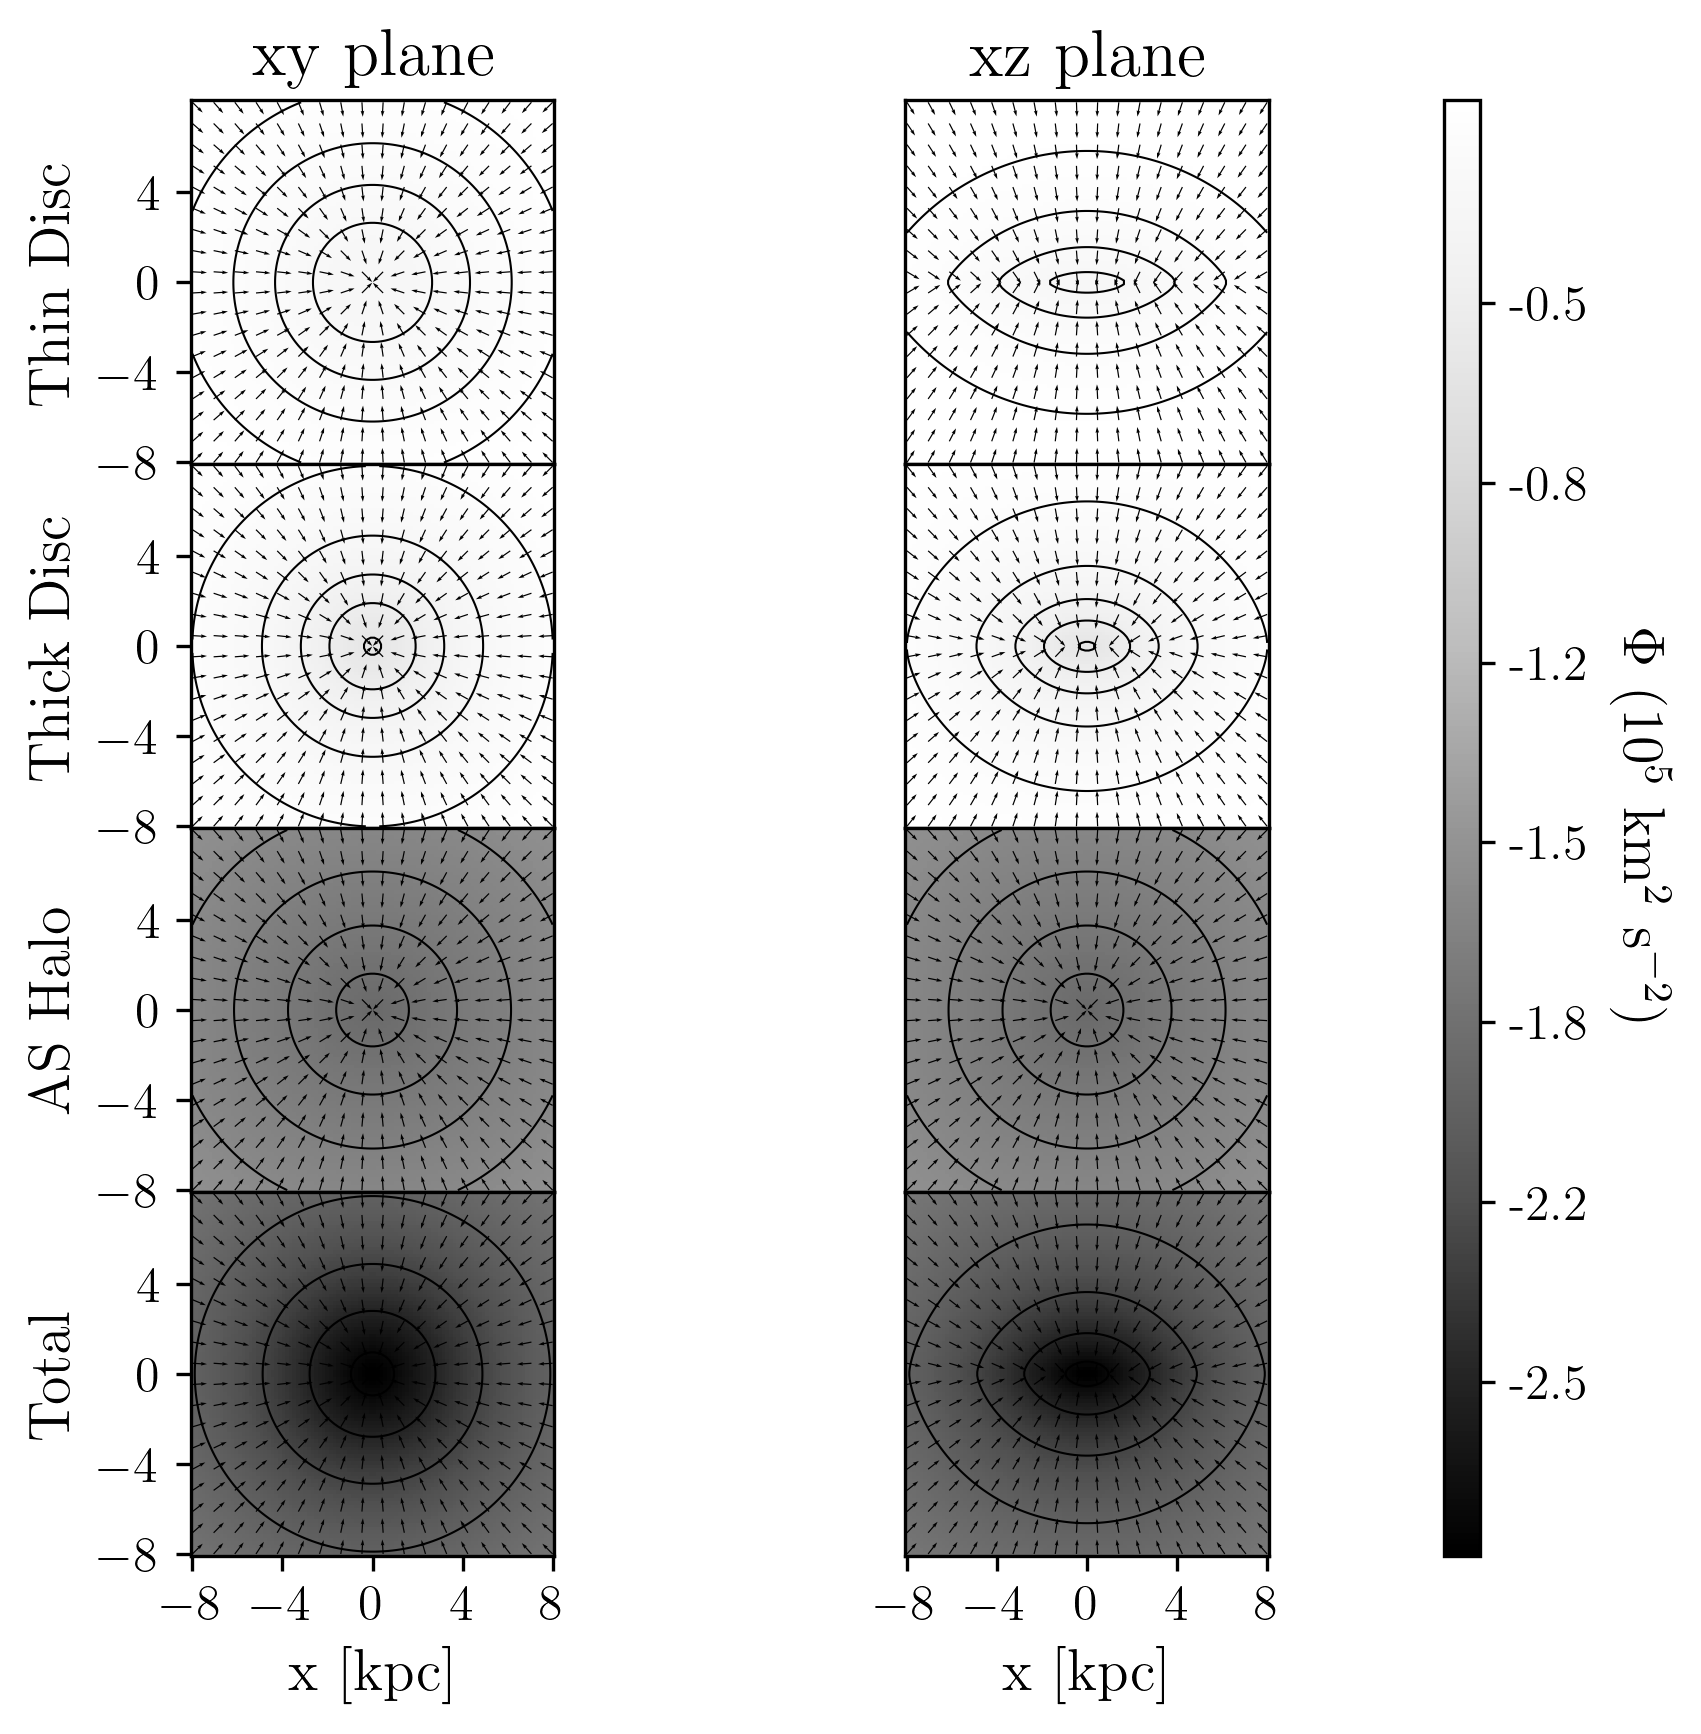
\includegraphics[width=\linewidth]{images/figure_pouliasis2017pii_potential_-8_8.png}
            \caption{The main potential used throughought the thesis}
        \end{figure}        
    

\section{The Implicit Physics}

    \subsection{The circular restricted three body problem}
        \begin{itemize}
            \item The Lagrange points
            \item Allowed regions 
        \end{itemize}

    \subsection{The tidal tensor}
        Tidal forces arise due to spatial variations in the gravitational field and are especially apparent when comparing the accelerations experienced by nearby particles. To explore this, consider a Taylor expansion of the gravitational potential of the primary, \(\Phi_g\), evaluated at the star's position \(\vec{x}_s\), relative to the secondary's position \(\vec{x}_c\):
        \begin{equation}
            \Phi_g\left(\vec{x}_s\right) \approx \Phi_g\left(\vec{x}_c\right) + \left[\nabla \Phi_g (\vec{x}_c)\cdot \Delta \vec{x}\right] + \left[\Delta \vec{x} \cdot \mathcal{D}^2\left(\Phi_g\right) \cdot \Delta\vec{x}\right],
        \end{equation}
        where \(\Delta \vec{x} = \vec{x}_s - \vec{x}_c\), and \(\mathcal{D}^2 \Phi_g\) is the Hessian matrix of second derivatives of the potential: \(\partial^2 \Phi/\partial x_i \partial x_j\).

        An equivalent expression can be derived by linearizing the gravitational force in a non-inertial frame co-moving with the secondary. Let us write Newton's second law for the star-particle and the secondary in an inertial frame:
        \begin{eqnarray}
            \vec{F}_s &= \nabla \Phi_c\left(\Delta \vec{x}\right) + \nabla \Phi_g\left(\vec{x}_s\right),\\
            \vec{F}_c &= \nabla \Phi_g\left(\vec{x}_c\right).
        \end{eqnarray}
        Then the relative acceleration of the star in the non-inertial frame is:
        \begin{eqnarray}
            \vec{f}_s &= \vec{F}_s - \vec{F}_c + \vec{F}_\mathrm{fictitious} \\
                    &= \nabla \Phi_c\left(\Delta \vec{x}\right) + \nabla \Phi_g\left(\vec{x}_s\right) - \nabla \Phi_g\left(\vec{x}_c\right) + \vec{F}_\mathrm{fictitious} \\
                    &\approx \nabla \Phi_c\left(\Delta \vec{x}\right) + \mathrm{Jac}\left(\nabla \Phi_g(\vec{x}_c)\right) \cdot \Delta \vec{x} + \vec{F}_\mathrm{fictitious},
        \end{eqnarray}
        where the last line uses a first-order Taylor expansion of the gravitational force field, valid under the assumption that \(|\Delta \vec{x}| \ll |\vec{x}_c|\). 

        The Jacobian of the gravitational field is equal to the Hessian of the potential, owing to the symmetry of second derivatives and the fact that \(\vec{g} = -\nabla \Phi_g\). This matrix, known as the \textit{tidal tensor} \(\mathcal{T}\), describes the linearized spatial variation of the gravitational field:
        \begin{equation}
            \mathcal{T} = -\mathcal{D}^2\Phi_g = \mathrm{Jac}(\nabla \Phi_g) = \left(\begin{matrix}
                \partial_x g_x & \partial_y g_x & \partial_z g_x \\
                \partial_x g_y & \partial_y g_y & \partial_z g_y \\
                \partial_x g_z & \partial_y g_z & \partial_z g_z 
            \end{matrix}\right).
        \end{equation}

        While the Hessian and Jacobian are formally equivalent, the Jacobian viewpoint offers a more geometric interpretation: it acts as a linear transformation on nearby displacements, mapping them to differences in acceleration. Diagonalizing the tidal tensor reveals the principal axes of tidal deformation. A positive eigenvalue corresponds to stretching along the associated eigenvector; a negative eigenvalue indicates compression. The magnitude gives the rate of stretching or compression.

        Finally, we note that although many relevant potentials exhibit spherical or cylindrical symmetry, Cartesian coordinates are preferred here. In curvilinear systems, computing the Jacobian or Hessian requires accounting for Christoffel symbols, which complicates the interpretation and computation.


        
        \subsubsection*{The Moon}
            Nothing clarifies the concept of tides like the most familiar example: the Moon. Tidal forces are invoked to explain a wide range of phenomena in the Earth-Moon system. The most relatable effect is, of course, the periodic variation in sea level on Earth. While accurately modeling these changes requires fluid dynamics—beyond the scope of this thesis—NASA provides several accessible explanations and visualizations at \href{https://science.nasa.gov/moon/tides/}{https://science.nasa.gov/moon/tides/}, including daily high and low tides, as well as spring and neap tides.

            Another key example is the tidal deformation of the Moon, which ultimately led to its tidal locking—explaining why we always see the same side of the Moon from Earth.

            A particularly insightful illustration is the angular offset between the Earth's tidal bulge and the Moon's position, caused by the Earth's rotation. This offset results in a torque that transfers angular momentum from the Earth's rotation to the Moon's orbit. As a consequence, Earth's rotation gradually slows while the Moon slowly recedes from Earth. Much of this behavior can be understood qualitatively using the tidal tensor for a Keplerian potential:
            \begin{equation}
                \mathcal{T}= -\frac{GM}{r^3}\left(\begin{matrix}
                    1-\frac{3x^2}{r^2} & -\frac{3xy}{r^2} & -\frac{3xz}{r^2} \\
                    -\frac{3yx}{r^2} & 1-\frac{3y^2}{r^2} & -\frac{3yz}{r^2} \\
                    -\frac{3zx}{r^2} & -\frac{3zy}{r^2} & 1-\frac{3z^2}{r^2}
                \end{matrix}\right),
            \end{equation}
            which has eigenvalues $2\frac{GM}{r^3}$, $-\frac{GM}{r^3}$, and $-\frac{GM}{r^3}$, with corresponding eigenvectors:
            \begin{equation}
                \vec{v}_1,\vec{v}_2,\vec{v}_3 = \dfrac{1}{r}\begin{bmatrix} x \\ y \\ z \end{bmatrix}, \dfrac{1}{r}\begin{bmatrix} -x \\ y \\ 0 \end{bmatrix}, \dfrac{1}{r}\begin{bmatrix} -x \\ 0 \\ z \end{bmatrix}.
            \end{equation}

            Notably, the first eigenvalue is positive and corresponds to a stretching deformation along the position vector. The other two are negative, representing compression in directions perpendicular to the stretching axis. These directions define a plane orthogonal to the Earth-Moon line. From this, several tidal effects become evident. For instance, the Earth's oceans stretch along the Earth-Moon axis due to the Moon's tidal forces. While the Sun also exerts tidal forces on Earth, their magnitude is weaker due to the $r^{-3}$ scaling with distance.

            When the Moon is either full or new, the Sun and Moon's tidal forces act constructively, leading to spring tides. At first and third quarters, they interfere destructively, causing neap tides. Additionally, Earth's tidal influence distorts the Moon from spherical symmetry into an ellipsoid. The Moon's most stable orientation is one where its longest axis aligns with the Earth-Moon line—resulting in tidal locking.

            A more quantitative treatment of these phenomena would require modeling the Moon's internal structure and Earth's ocean dynamics—well beyond the gravity-only scope of this thesis. However, we can still explore one instructive effect: how solar tidal forces \textit{perturb} the Moon's orbit away from the idealized two-body Earth-Moon configuration. Figure~\ref{fig:moon_tidal_simulation} shows a toy model comparing two scenarios. In both, I used initial conditions based on JPL NASA ephemerides (citation needed) and integrated two sets of equations of motion.

            In the first scenario, the Moon's motion is governed by the two-body Earth-Moon problem with a rotating reference frame correction:
            \begin{equation}
                \ddot{\vec{r}} = -\frac{GM_\oplus}{r^3}\vec{r} - \omega_\oplus \times \left(\omega_\oplus \times \vec{r}_\oplus\right),
            \end{equation}
            while in the second, we include the effect of solar tidal forces:
            \begin{equation}
                \ddot{\vec{r}} = -\frac{GM_\oplus}{r^3}\vec{r} - \omega_\oplus \times \left(\omega_\oplus \times \vec{r}_\oplus\right) -\frac{GM_\odot}{r_\oplus^3}
                \left(\begin{matrix}
                    1-\frac{3x^2}{r_\oplus^2} & -\frac{3xy}{r_\oplus^2} & -\frac{3xz}{r_\oplus^2} \\
                    -\frac{3yx}{r_\oplus^2} & 1-\frac{3y^2}{r_\oplus^2} & -\frac{3yz}{r_\oplus^2} \\
                    -\frac{3zx}{r_\oplus^2} & -\frac{3zy}{r_\oplus^2} & 1-\frac{3z^2}{r_\oplus^2}
                \end{matrix}  \right) \cdot \vec{r},
            \end{equation}
            where $r_\oplus$ is the Earth's position relative to the Sun, $\vec{r}$ is the Moon's position relative to Earth, $M_\odot$ is the mass of the Sun, and $M_\oplus$ is the mass of the Earth. The coordinates $x, y, z$ refer to the components of Earth's heliocentric position.

            
            
            \begin{verbatim}
            VIDEO: moon_tidal_simulation.mp4
            \end{verbatim}

            \begin{figure}
                \centering
                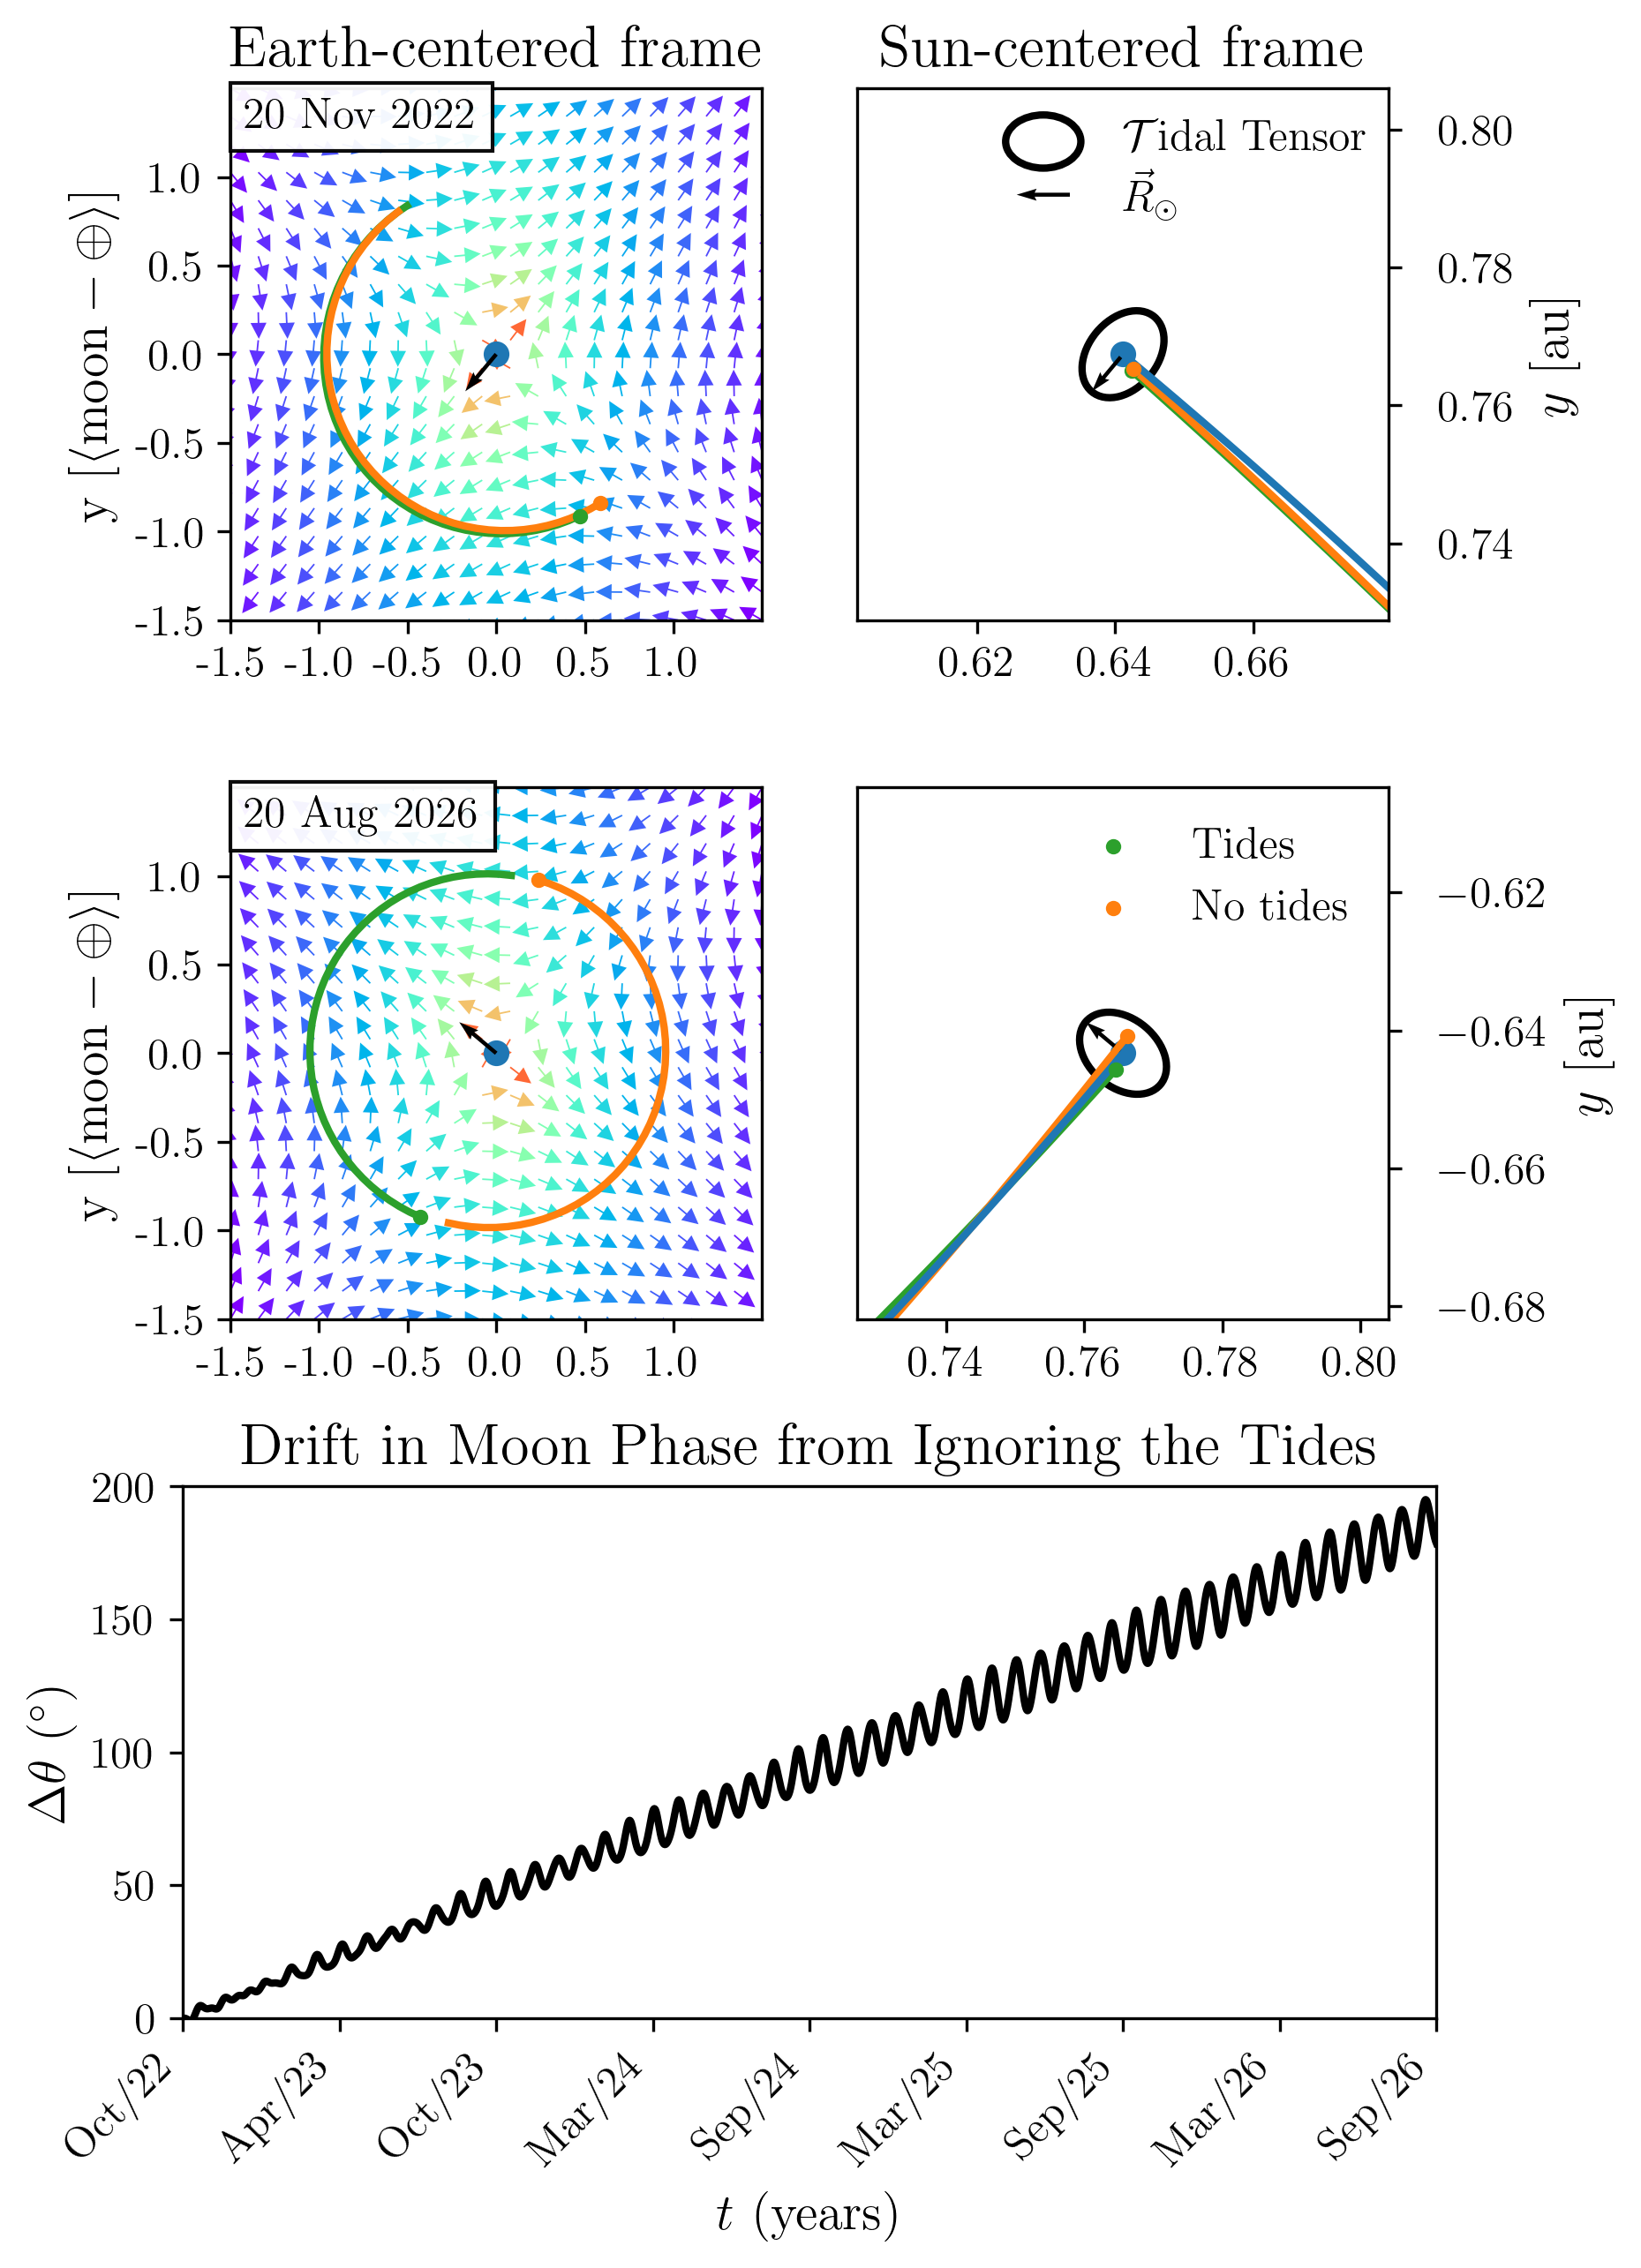
\includegraphics[width=\linewidth]{images/moon_tidal_simulation.png}
                \caption{An illustrative experiment demonstrating the effect of the Sun's tidal field. The left panels show the tidal field, and the right panels show two snapshots of the Moon's orbital trajectory. The green curve corresponds to the solution of Eq.~\textbf{XXX}, which includes the Sun's tidal effects, while the orange curve corresponds to the simpler two-body problem that neglects them. The black ellipse represents the tidal ellipsoid, whose major axis remains aligned with the Sun's position vector relative to the Earth. The bottom panel shows the accumulated phase difference between the two solutions. Neglecting solar tides causes the predicted Moon orbit to drift ahead of the more accurate trajectory. With about three to four years, the two body predicted solution would off by half a moon phase.
                }\label{fig:moon_tidal_simulation}
            \end{figure}

        \subsubsection*{Tides in the Galaxy}
            
            How the tidal field varies throughout the Galaxy by evaluating the tidal tensor along different orbits and in different mass models. In the Milky Way, the disk, bulge, and halo each contribute differently to the tidal forces experienced by a globular cluster. The Miyamoto-Nagai disk produces strong, rapidly varying tidal fields near the Galactic plane, leading to phenomena such as disk shocking when clusters cross the disk. The Martos halo, on the other hand, provides a more slowly varying, generally weaker tidal field at large Galactocentric radii.

            The strength and orientation of the tidal field at a cluster's location determine both the rate at which stars are stripped and the geometry of the resulting stellar streams. For example, clusters on eccentric or inclined orbits experience time-dependent tidal forces, with strong compressive shocks during disk crossings and enhanced stretching near pericenter. The eigenvalues and eigenvectors of the tidal tensor at each point along the orbit reveal the principal axes of stretching and compression, which in turn set the directions along which stars are most likely to escape.

            By computing the tidal tensor for the Miyamoto-Nagai disk and Martos halo potentials, as shown below, we can visualize and quantify these effects. The following figures illustrate how the tidal field evolves for representative orbits, highlighting the interplay between the cluster's trajectory and the Galactic mass distribution. This analysis underpins our understanding of stream formation and the morphological diversity of observed tidal tails.

            We can construct the tidal tensor for the Miyamoto-Nagai potential. First, it is convenient to non-dimensionalize the potential. Below, we normalize the potential by the total mass and gravitational constant, $\Phi\prime = \Phi / (GM)$, and each distance by the characteristic length of the disk, $x' = x/a$, $b' = b/a$. For clarity, we omit the prime notation in what follows. The dimensionless potential then becomes:            
            \begin{eqnarray}
                \Phi   &= \frac{1}{D},\\
                D       &= \sqrt{x^2 + y^2 + \beta^2(z)},\\
                \beta(z)   &= 1 + \sqrt{z^2 + b^2}.
            \end{eqnarray}
                % \beta^{\prime}(z) &= \frac{z}{\sqrt{z^2 + b^2}}\\
                % \beta^{\prime\prime}(z)  &= \frac{b^2}{\left(z^2 + b^2\right)^{3/2}}
            % \end{eqnarray}
            The dimensionless tidal tensor is then: 
            \begin{equation}
                \mathcal{T}=-\frac{1}{D^3}\left(\begin{matrix}
                    1-\frac{3x^2}{D^2} & -\frac{3xy}{D^2} & -\frac{3x\beta \beta'}{D^2} \\
                    \dots & 1-\frac{3y^2}{D^2} & -\frac{3y\beta \beta'}{D^2} \\
                    \dots & \dots & \beta'^2 + \beta \beta'' -\frac{3\left(\beta\beta'\right)^2}{D^2}
                \end{matrix}\right).
            \end{equation}             
            We immediately notice that, due to the cylindrical symmetry, the eigenvectors are not as simple as in the spherical case. As long as $\beta'^2 + \beta \beta'' -\frac{3\left(\beta\beta'\right)^2}{D^2} \neq 1-\frac{3z^2}{D^2}$, the three eigenvectors are no longer simply (1) parallel to the position vector and (2) the other two spanning the plane perpendicular to it. Instead, the exact orientation of all three eigenvectors depends on the cluster's position in the galaxy. Note that if $z=0$, we recover the stretching eigenvector being parallel to the position vector, although the orientations of the eigen vector are fixed as the compression axes are not the same in magnitude. If, we $b=0$, then we recover spherical symmetry and the compression eigenvalues are the same in magnitude.

            \begin{verbatim}
            VIDEO: tidal_deformation_ellipsoid.mp4
            \end{verbatim}

            Below I have prepared some selected orbits to demonstrate the variety of shocks and tidal forces than can influence a globular cluster system. 
            
            \begin{figure}
                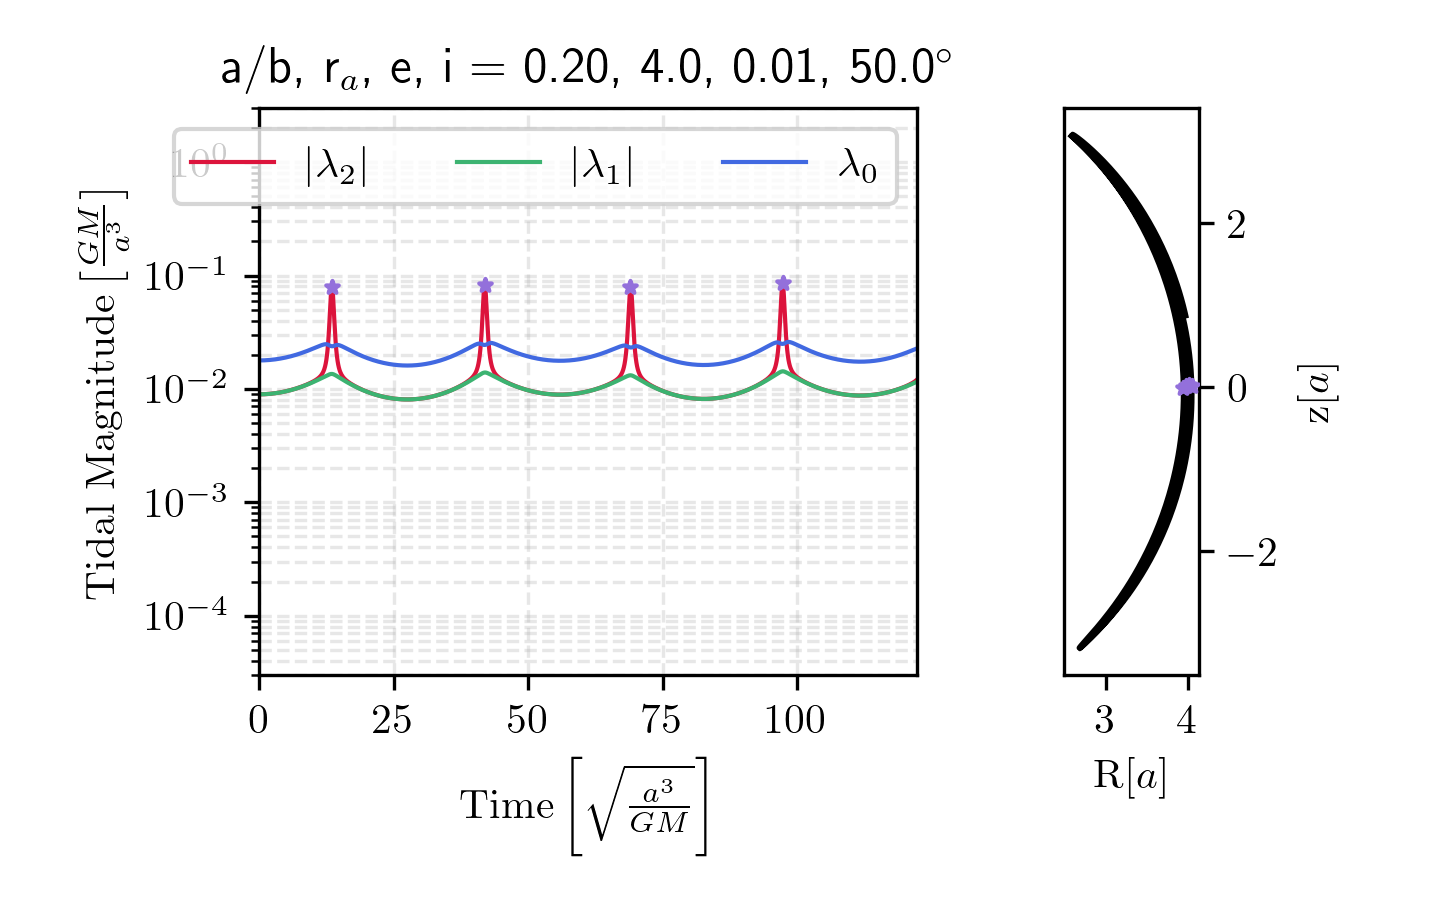
\includegraphics[width=\linewidth]{images/miyamoto_disc_shocks_ab_rp_e_i_0.20_4.0_0.01_50.0.png}
                \caption{Tidal forces on an inclined yet non-eccentric orbit. Disk shocks are present, yet there is no tidal stretching from pericenter passages. \textbf{Left}: The three eigenvalues of the tidal tensor matrix are plotted against time. Both the forces and time are normalized to the characteristic values of the Miyamoto-Nagai model, where $a$ is the radial scale length and $M$ is the total mass of the system. The red and green curves correspond to the two compressive axes, while the blue curve shows the magnitude of the stretching axis. The parameters listed at the top describe the orbit: the ratio of cylindrical to vertical scale lengths, the apocenter distance, the eccentricity, and the initial orbital inclination. \textbf{Right}: The orbit is shown in the meridional plane. The purple stars indicate disk crossing events and correspond to the peaks in the magnitude of the eigenvalues. }
                \label{fig:miyamoto_disc_shocks_circular_inclined_orbit}
            \end{figure}


            \begin{figure}
                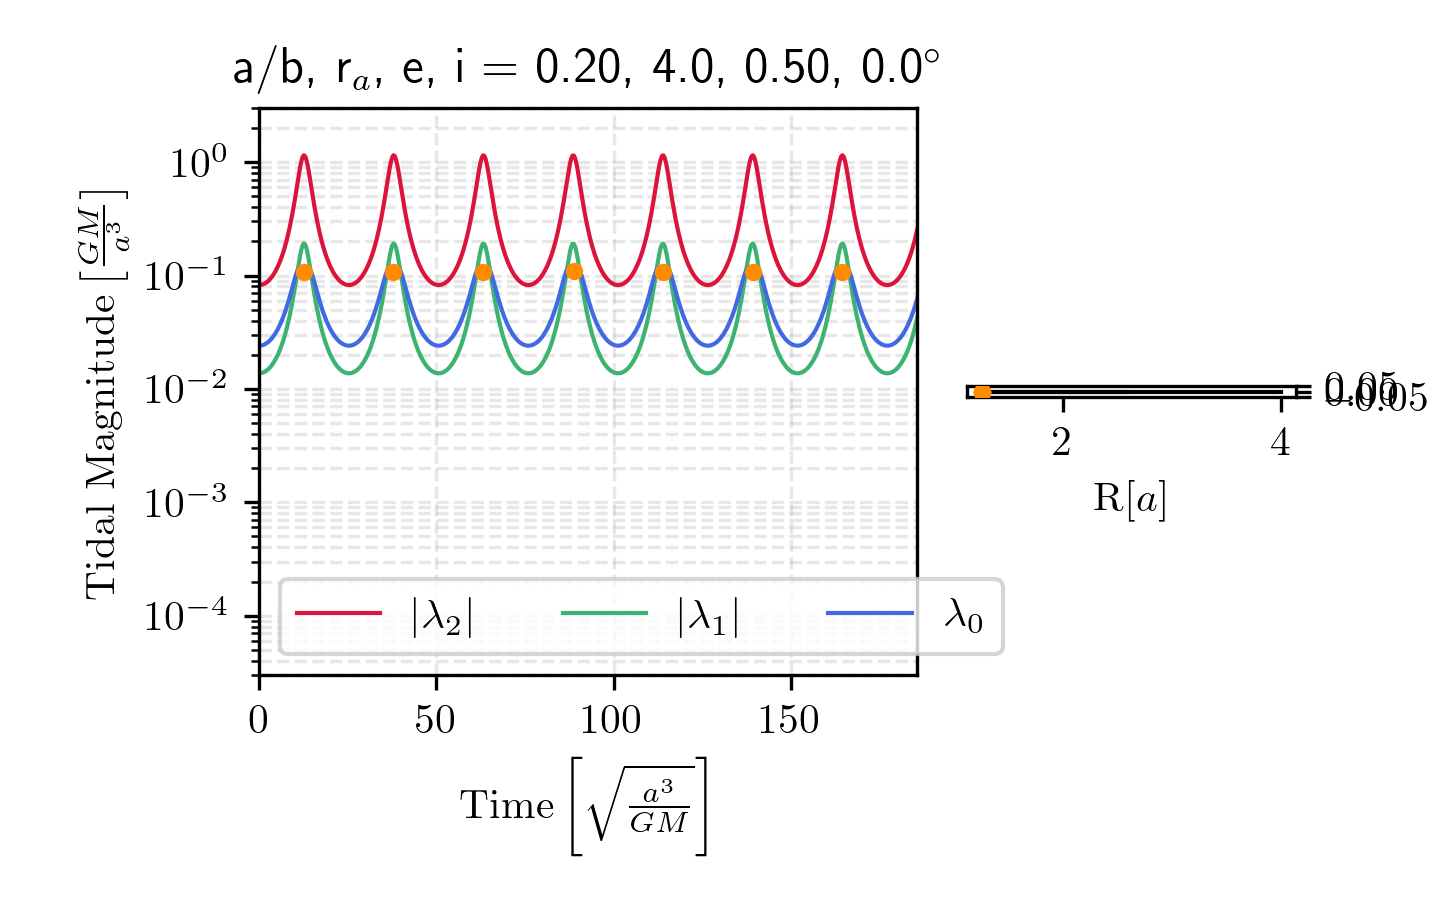
\includegraphics[width=\linewidth]{images/miyamoto_disc_shocks_ab_rp_e_i_0.20_4.0_0.50_0.0.png}
                \caption{Evolution of the tidal eigenvectors for an eccentric, non-inclined orbit, resulting in a compressed meridional plane. Orange dots mark the pericenter passages. Since the cluster remains confined to the plane, no disk shocks occur.}
                \label{fig:miyamoto_disc_shocks_circular_inclined_orbit}
            \end{figure}

            \begin{figure}
                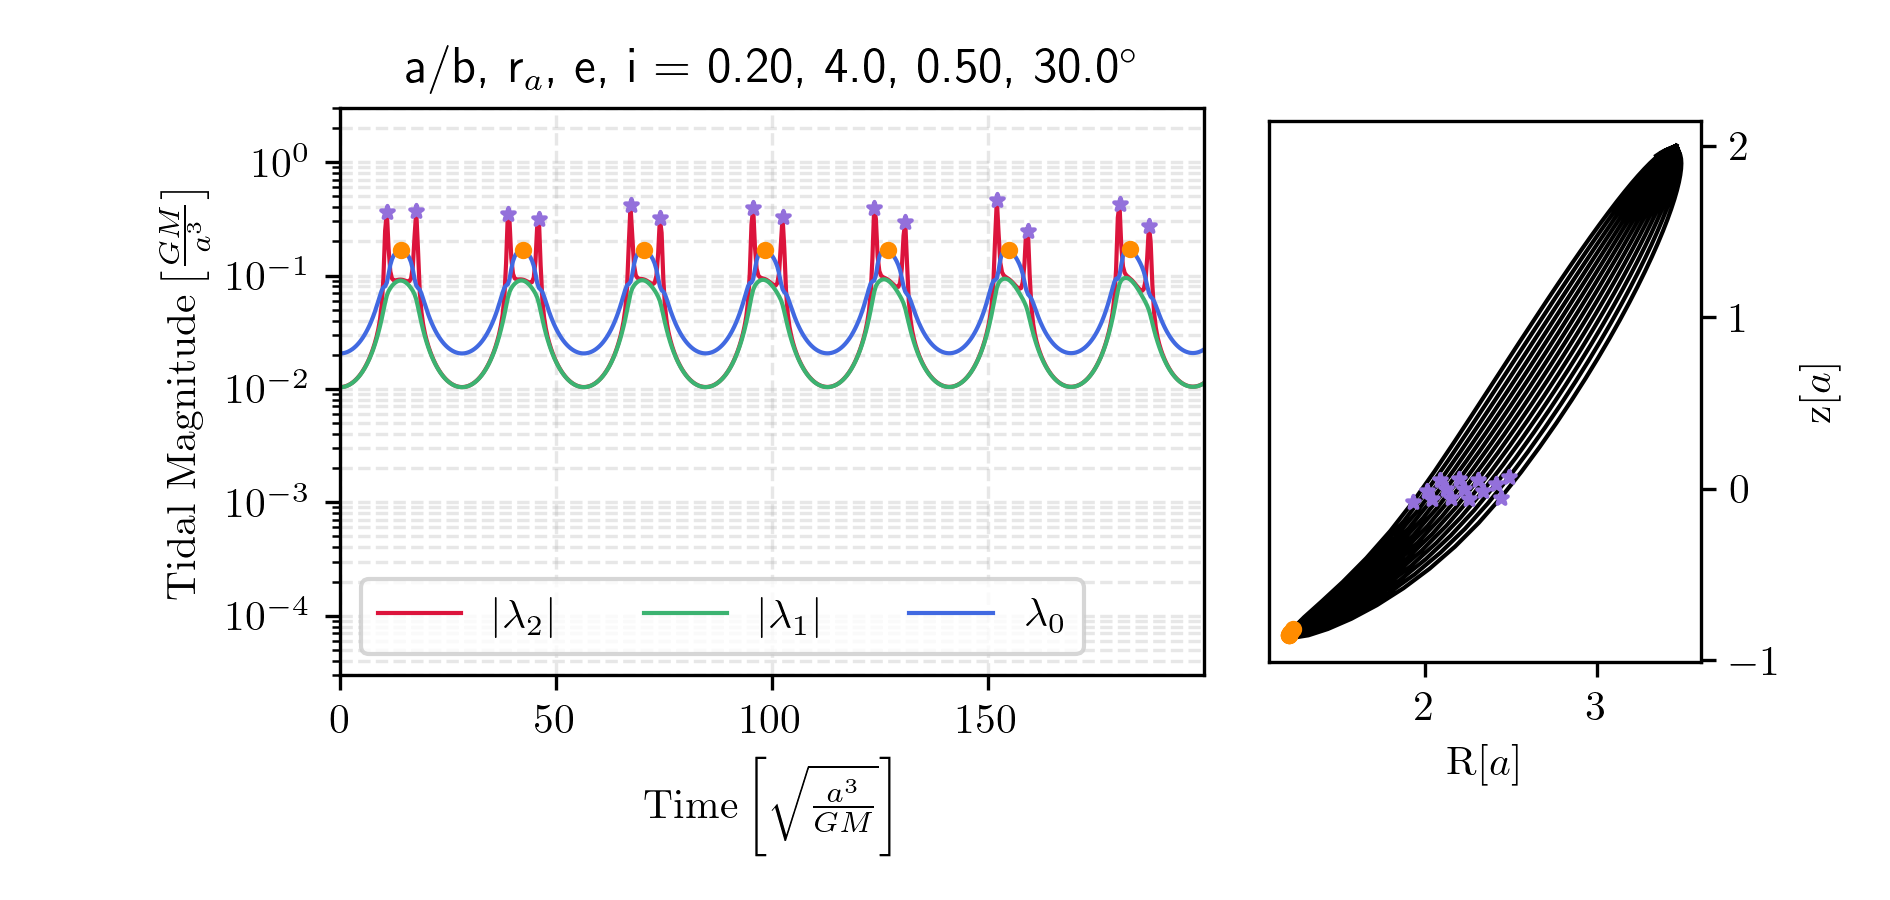
\includegraphics[width=\linewidth]{images/miyamoto_disc_shocks_ab_rp_e_i_0.20_4.0_0.50_30.0.png}
                \caption{An inclined, eccentric orbit in which the frequencies in both the $R, p_R$ and $z, p_z$ planes are nearly resonant. The cluster crosses the disk just before and just after each pericenter passage. This is the same orbit as the video presented in this section that is available in the online version.}
                \label{fig:miyamoto_disc_shocks_responant_R_z}
            \end{figure}
            
            \begin{figure}
                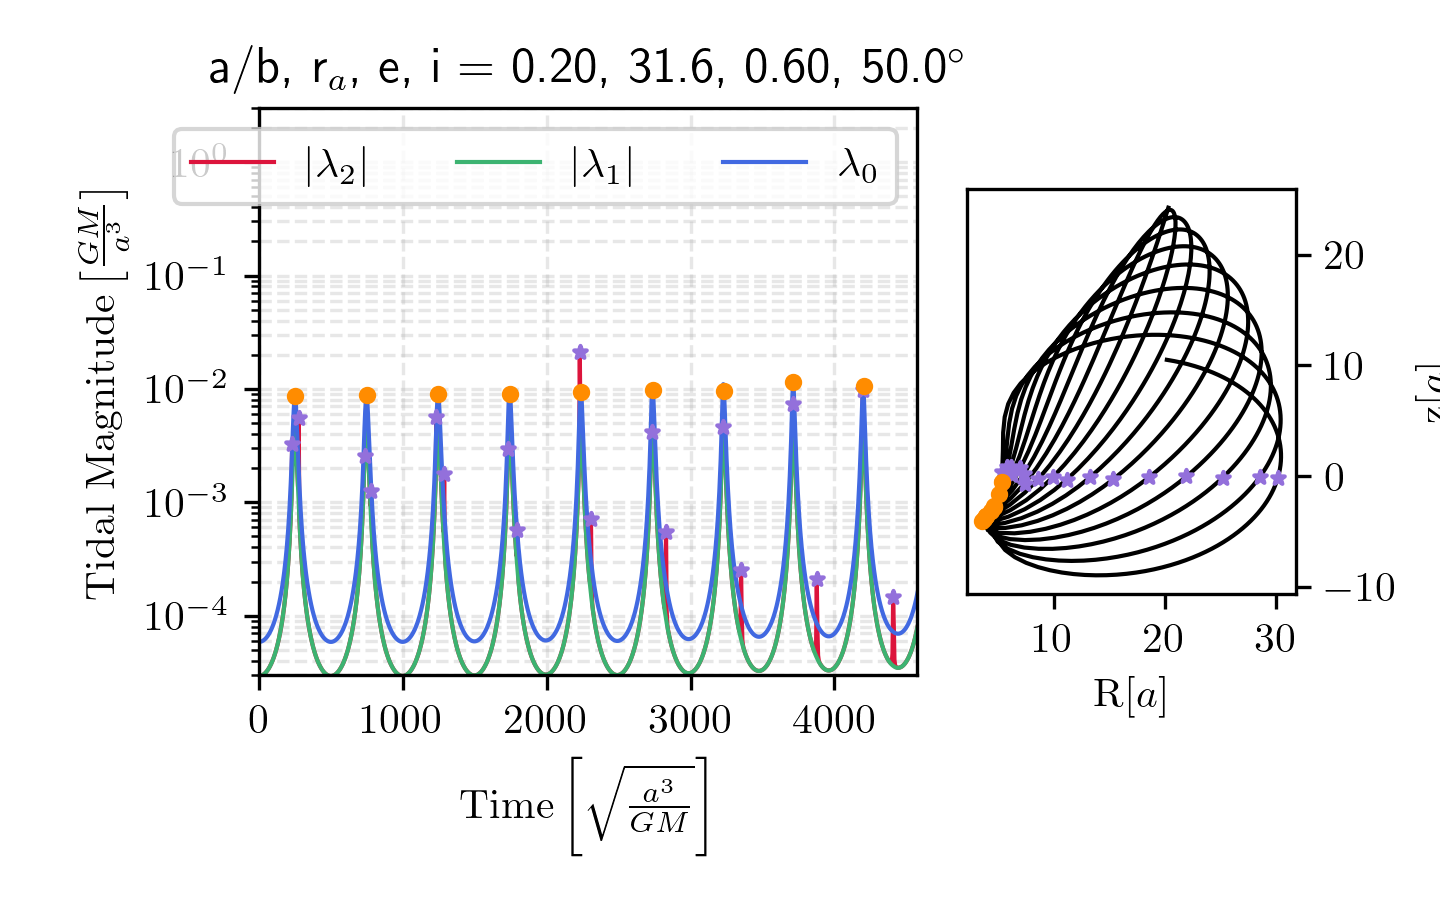
\includegraphics[width=\linewidth]{images/miyamoto_disc_shocks_ab_rp_e_i_0.20_31.6_0.60_50.0.png}
                \caption{An eccentric, inclined orbit with a large apocenter. As the cluster evolves through phase space, disk crossings that occur farther out happen at steeper angles and in lower-density regions, reducing the strength of the resulting disk shocks. In contrast, crossings near pericenter remain strong. Because this orbit has higher energy than the previous cases, the overall magnitude of the tidal forces is lower. }
                \label{fig:miyamoto_disc_shocks_big_apocenter}
            \end{figure}
            
            \begin{figure}
                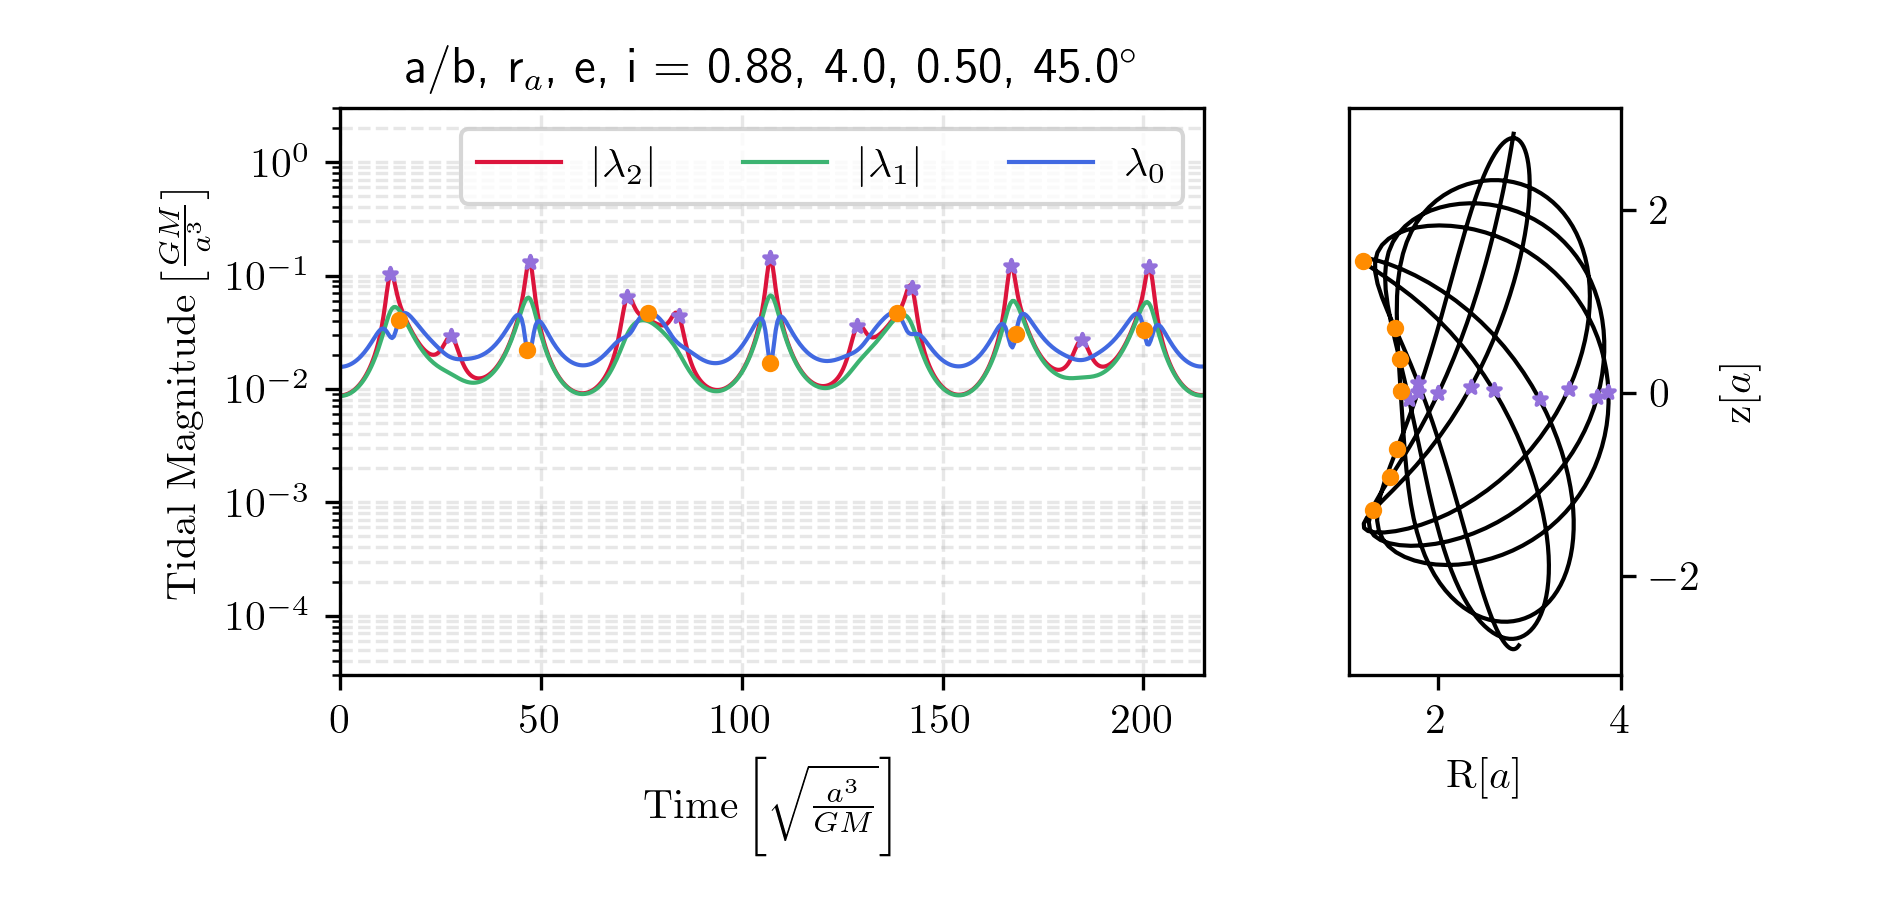
\includegraphics[width=\linewidth]{images/miyamoto_disc_shocks_ab_rp_e_i_0.88_4.0_0.50_45.0.png}
                \caption{Eccentric and inclined orbit in a weak disk. The ratio of the cylindrical scale length  to characteristic height (a/b) is close to 1. The disk crossings still produce significant tidal compression, but the resulting shocks are broader.}
                \label{fig:miyamoto_disc_shocks_weak_shocks}
            \end{figure}


   
        \subsubsection*{Interesting case}

            The Marto's halo has this mass distribution:
            
            \begin{equation}
                M'_\text{enc}(s) = \frac{s^\gamma}{1+s^{\gamma-1}}
            \end{equation}
            The dimensionless tidal tensor is thus: 
            \begin{equation}
                \mathcal{T'}_{i,j}= -\frac{M'_\text{enc}(s)}{s^3}\left(\begin{matrix}
                    1-\frac{x^2}{s^2}f(s) & -\frac{xy}{s^2}f(s) & -\frac{xz}{s^2}f(s) \\
                    -\frac{yx}{s^2}f(s) & 1-\frac{y^2}{s^2}f(s) & -\frac{yz}{s^2}f(s) \\
                    -\frac{zx}{s^2}f(s) & -\frac{zy}{s^2}f(s) & 1-\frac{z^2}{s^2}f(s)
                \end{matrix}\right)
            \end{equation}  
            where 
            \begin{equation}\label{eq:martos_f_s}
                f(s) = 2-\frac{\gamma-1}{1+s^{\gamma-1}}
            \end{equation}

            There is an interesting area in the parameter space where the tidal forces would impede creating stellar streams instead of making them, as shown in Fig.~\ref{fig:martos_tidal_field_small_r}.

            Taking the Martos tidal tensor in Eq.~\ref{eq:martos_f_s}, we can see that for $\gamma > 3$ and $s \ll  1$, then $f(s)< 0$. Physically, this would be a sphere whose density increases with distance. This is not natural, as, in general, gravity sends the more massive objects towards the center. However, it's fun to indulge in this situation to learn some insight about the flexibility of tidal fields. The consequence of $f(s)< 0$ is that all terms in the tidal tensor are negative, which means that the force is compressive everywhere. Consequently, no stars escape from the cluster. 

            In Fig.~\ref{fig:martos_tidal_field_small_r}, I present a small experiment demonstrating the consequence of such a tidal force on a globular cluster, which is that no tidal stream forms. Briefly, I created a plummer sphere of $10^6$~M$_\odot$ and half mass radius 20~pc and evolved it in a Martos halo potential of mass parameter $10^{12}$~M$_\odot$ a characteristic radius of $30$~kpc. Each cluster was placed at the same initial conditions, a distance of 1/4 the scale radius from the center of the potential. The initial velocity was made perpendicular to the position vector with a speed of $(1-e)v_\textrm{c}$. This is a pseudo-eccentricity, which was added to have a non-circular orbit to demonstrate how the trajectories change in the two cases. The top panel uses a $\gamma$ of 2.02, which is the same value in the model where the halo was originally presented, and the value I employ in this thesis. Next, the bottom panel uses $\gamma$ of 4.5, which corresponds to a density profile where $\rho(r) \propto r^{1.5}$. 

            To get a feel for the strength of the tidal stretching and compression, I show a circle and the resulting ellipse after applying the tidal deformation. I computed the coordinates of the ellipse by adding $\vec{Ell} = \vec{C} + \frac{1}{2} t_\textrm{char}^2 \mathcal{T}\cdot \left(\vec{C} - \vec{r_o}\right)$. This way, force can be mapped to position space, and the strengths of the tidal forces can be seen visually. The characteristic time, $t_\textrm{char}$, was set to $\frac{1}{10} 2\pi r_\textrm{halo} / v_\textrm{c}$. 
            
            \begin{figure}
                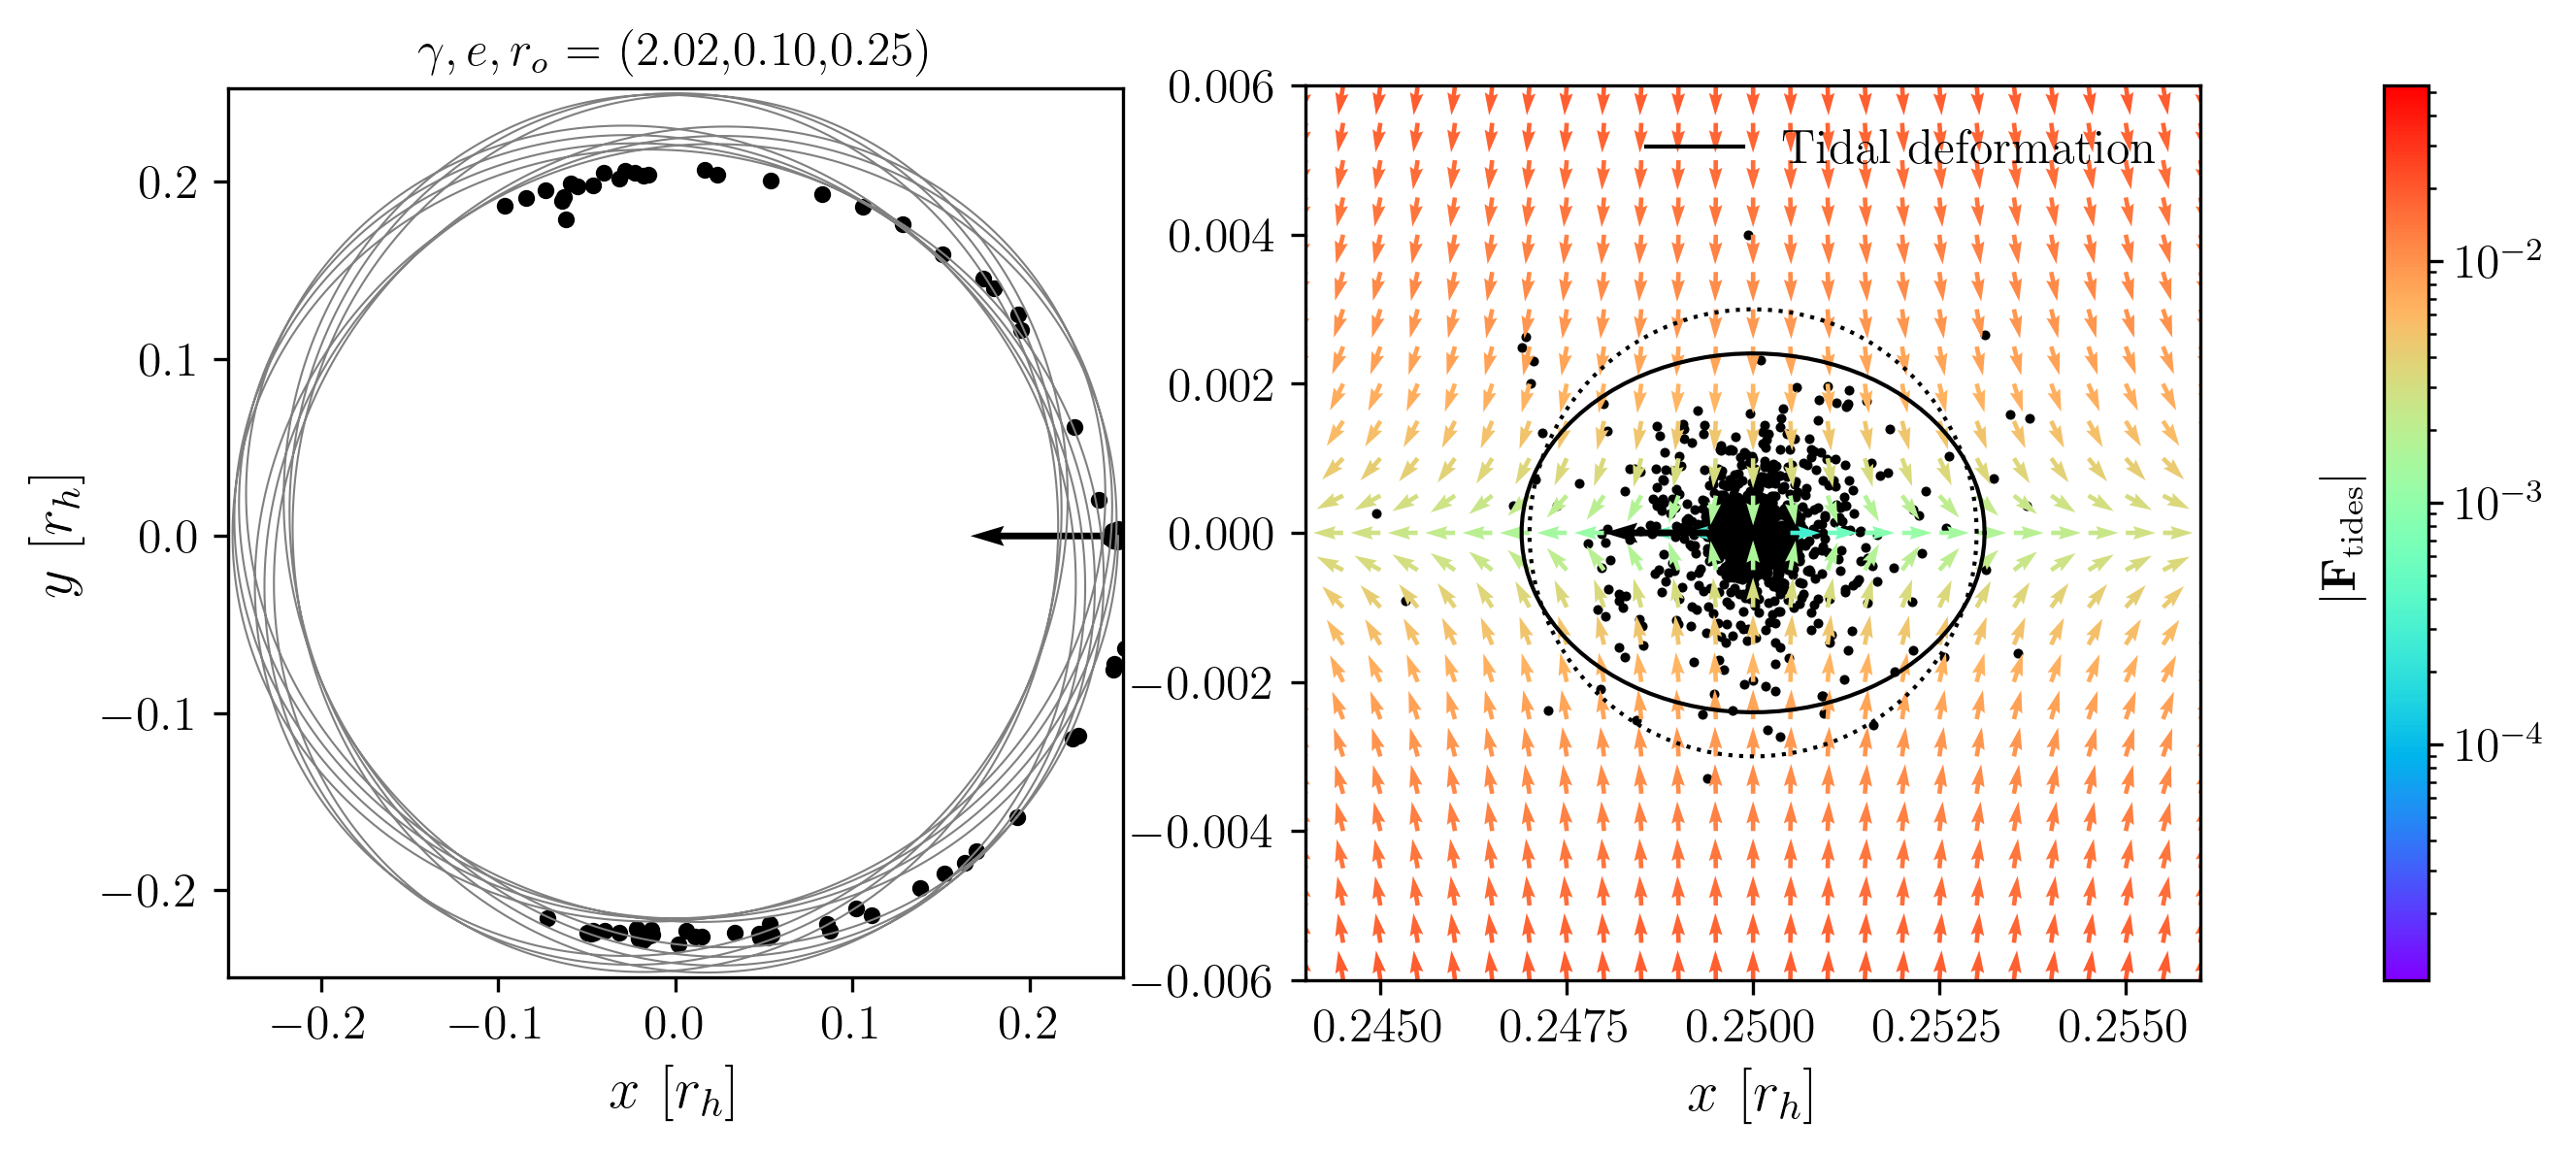
\includegraphics[width=\linewidth]{images/martos_tidal_field_202_10_25.png}
                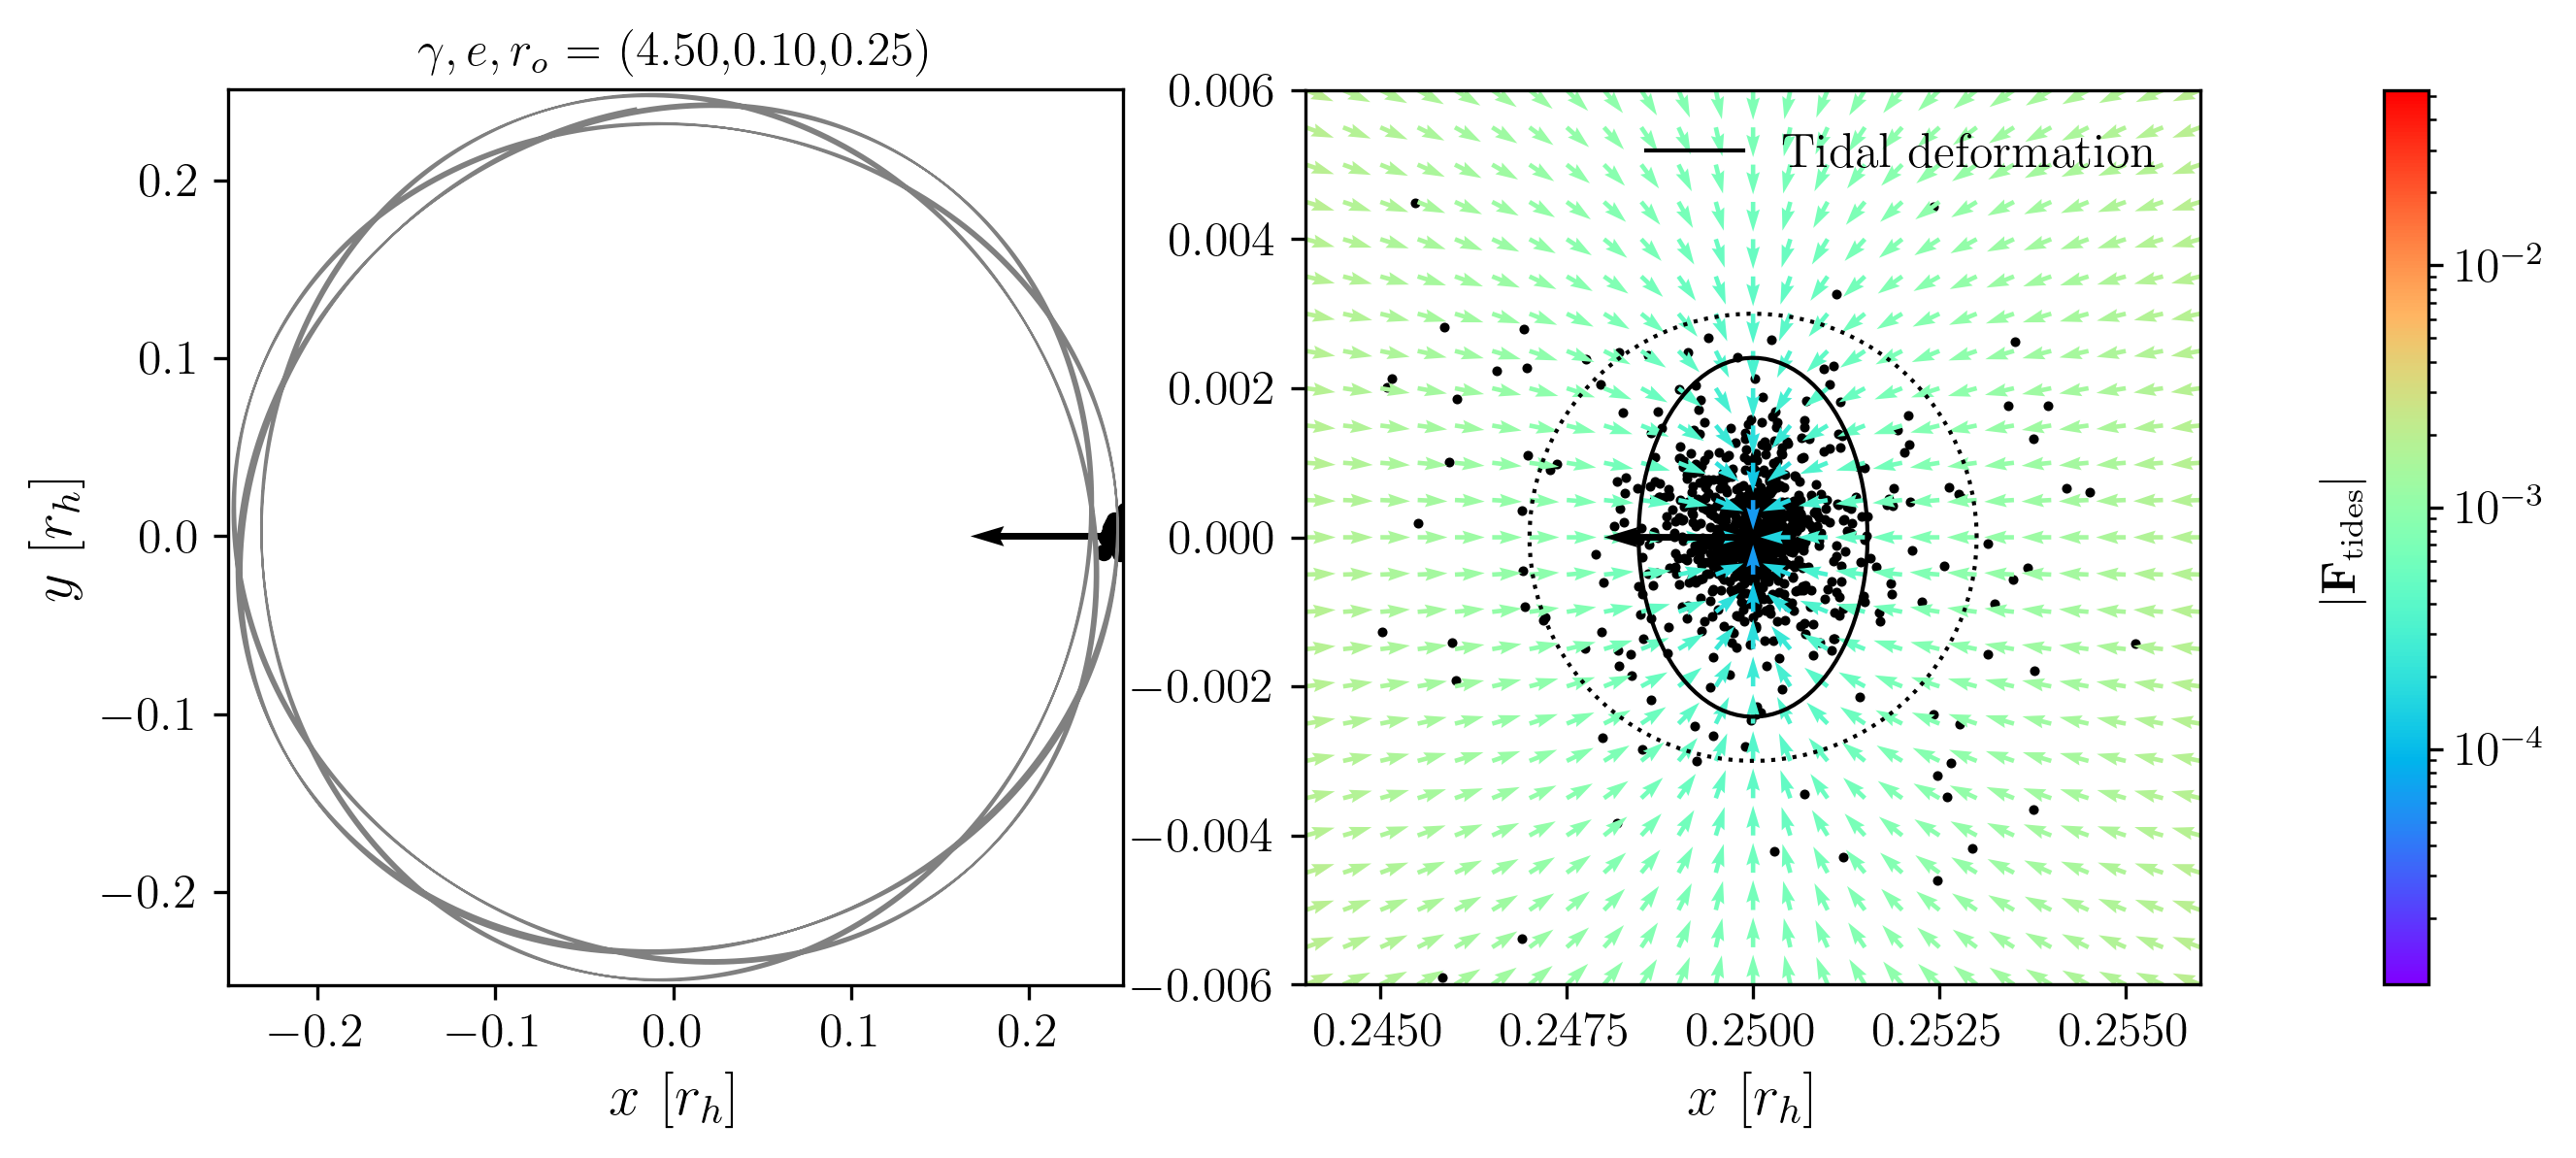
\includegraphics[width=\linewidth]{images/martos_tidal_field_450_10_25.png}
                \caption{The plots show two low-resolution streams (N = 1000) created by dissolving a Plummer sphere in the Martos halo potential. The units are scaled to the halo's characteristic radius. Gamma is the mass exponent and is the sole variable between the two simulations. The panels on the left show the orbit in gray and the stars in black. The black arrow points towards the center of the potential. The panels on the right show the tidal field, which is the tidal tensor evaluated at each position in space. The gray dotted circle is plotted with an arbitrary radius and is deformed by the tidal field into a black ellipse.}
                \label{fig:martos_tidal_field_small_r}
            \end{figure}

            \begin{figure}
                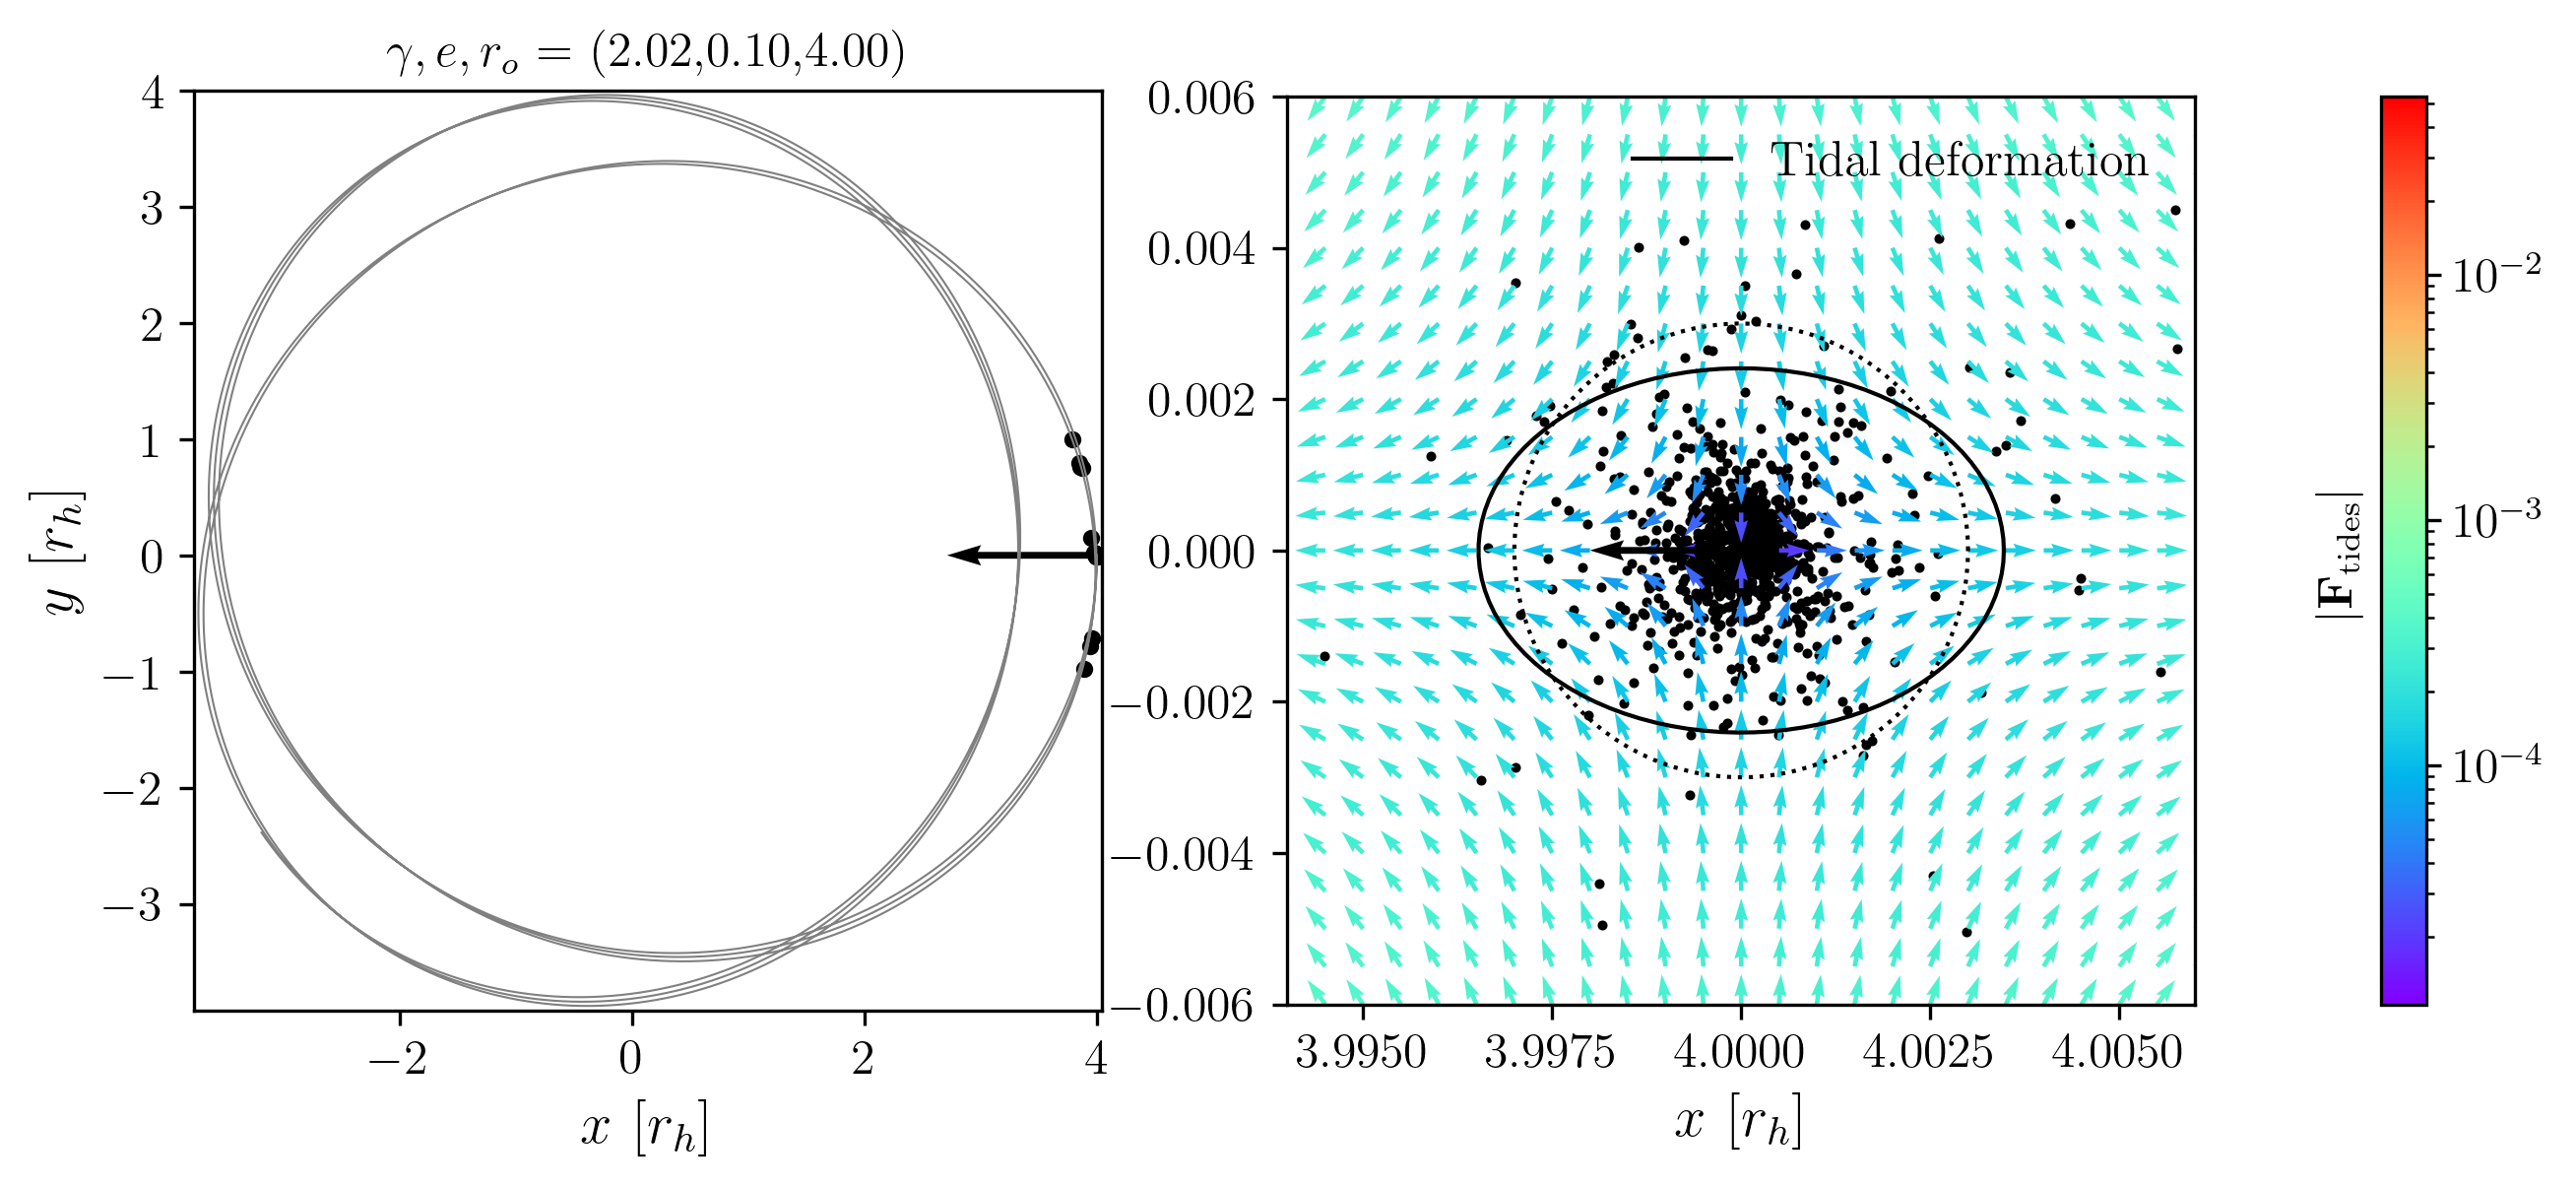
\includegraphics[width=\linewidth]{images/martos_tidal_field_202_10_400.png}
                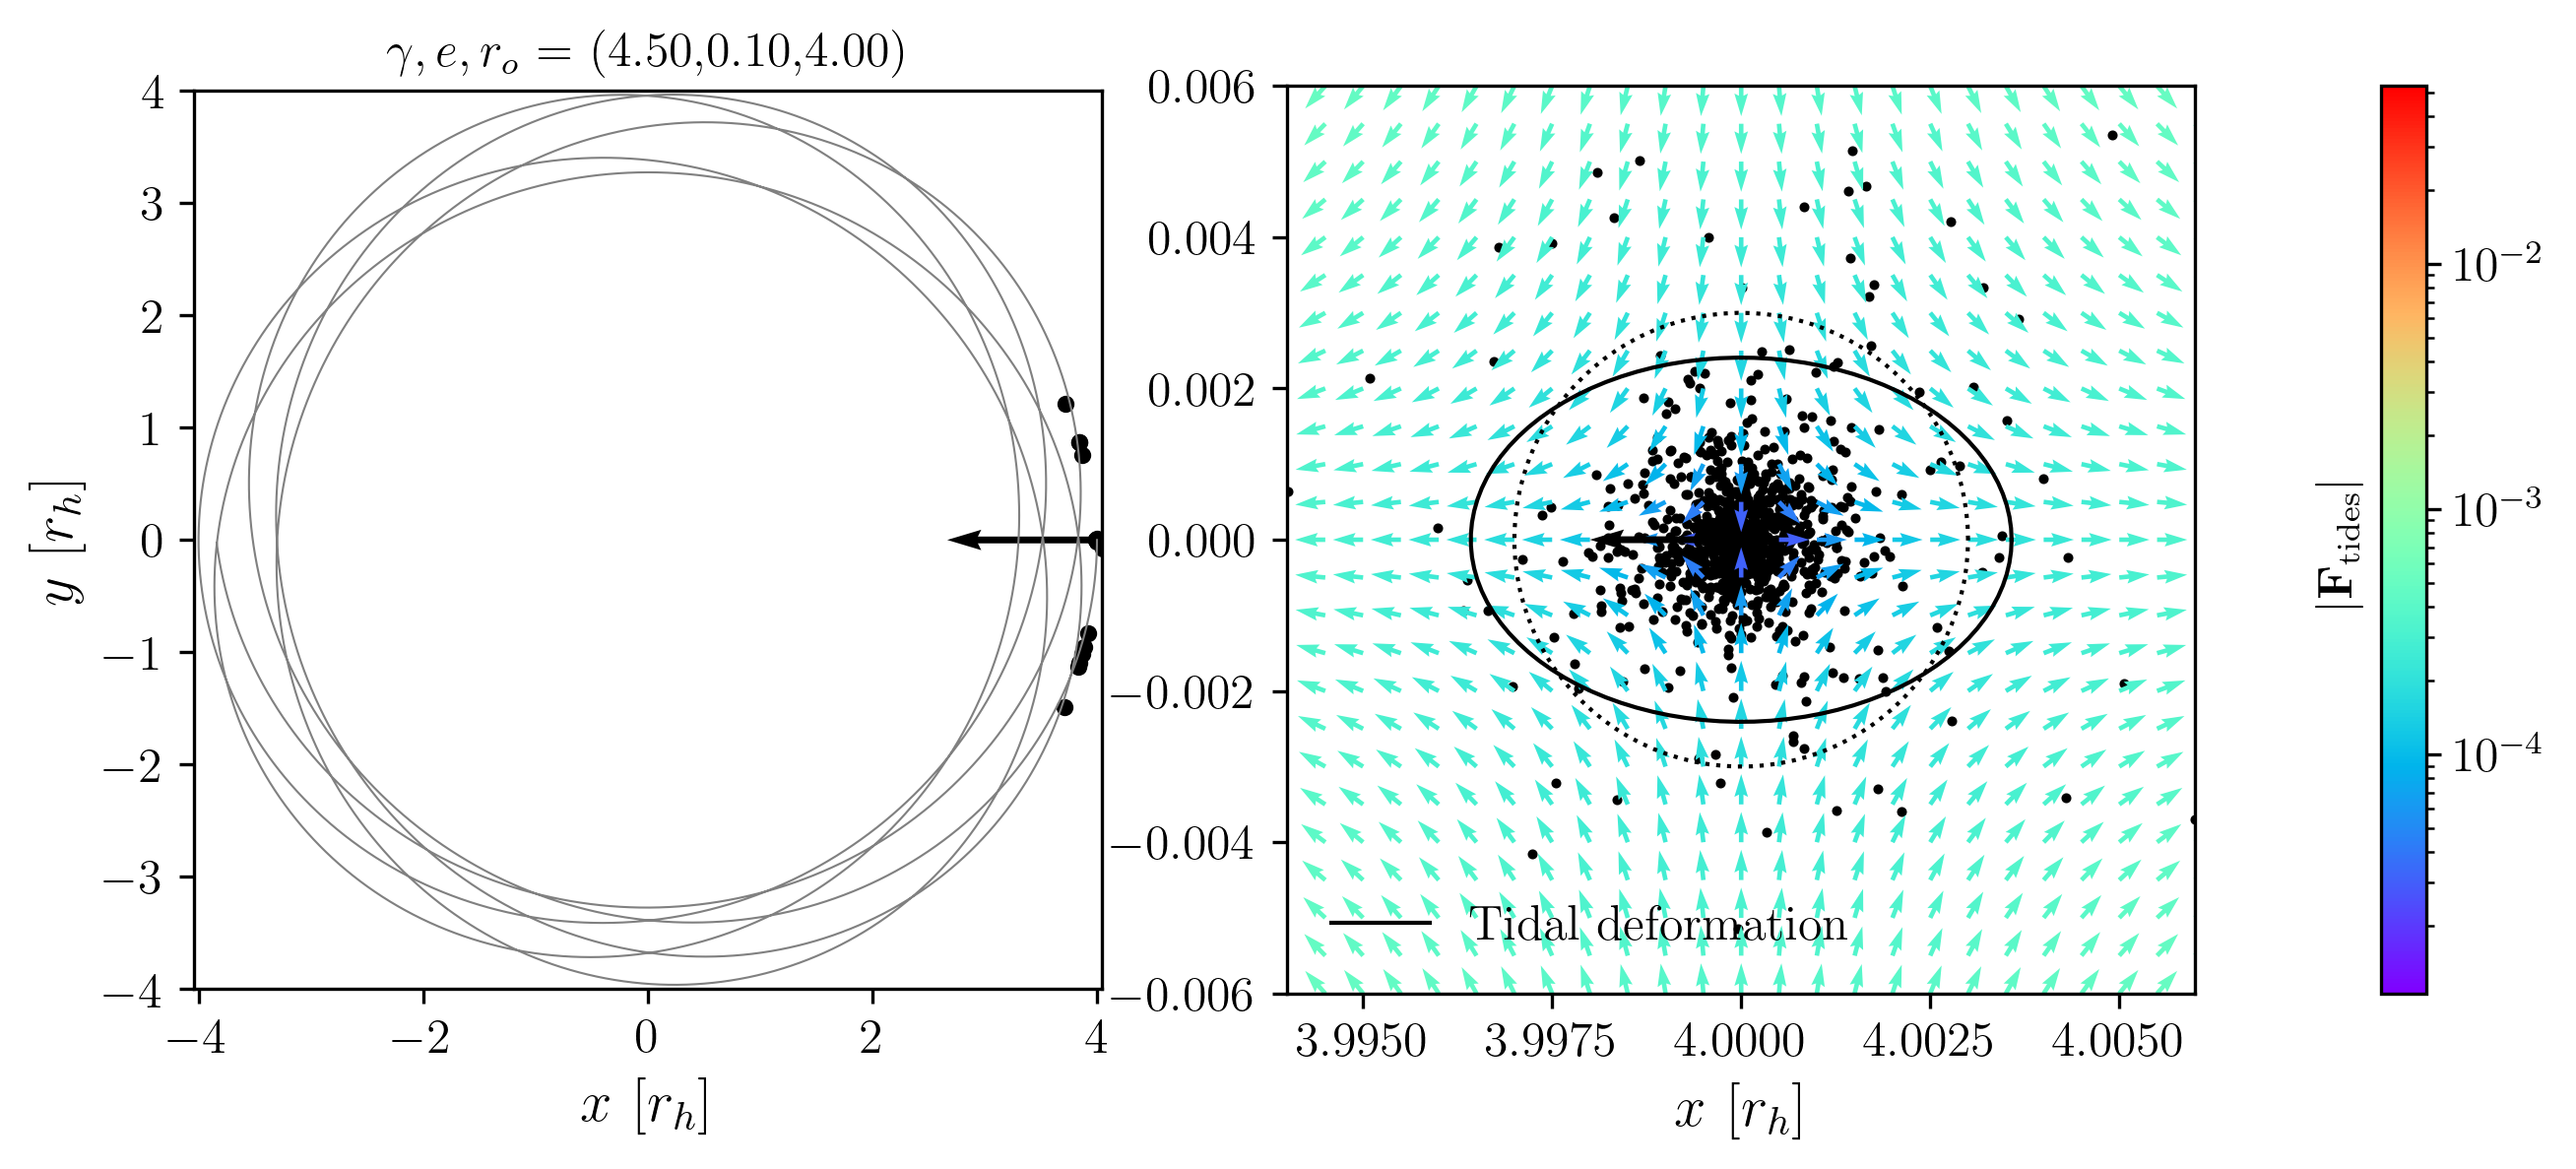
\includegraphics[width=\linewidth]{images/martos_tidal_field_450_10_400.png}
                \caption{The same experiment as Fig.~\ref{fig:martos_tidal_field_small_r}, but the cluster was placed at a larger distance of 4 $r_\textrm{halo}$, since we are beyond the characteristic radius, the tidal fields are the same, despite the different exponents $\gamma$.}
                \label{fig:martos_tidal_field_big_r}
            \end{figure}

            In the case of Fig.~\ref{fig:martos_tidal_field_big_r}, the tidal field returns to the typical situation where one axis is compressive and the other stretches. Notice how the deformations are similar in magnitude, while in the case of $\gamma=2.02$ for the top panel of Fig.~\ref{fig:martos_tidal_field_small_r}, the compression is stronger than the expansion. Both of these are different than the keplerian tidal deformation where the stronger deformation is stretching and whose axis is parallel to the position vector. 






    \subsection{Phase mixing}
        \textit{Phase mixing} is a direct consequence of Liouville's theorem, which itself follows from the collisionless Boltzmann equation. Liouville's theorem states that the infinitesimal volume element in phase space is preserved under Hamiltonian evolution. In other words, as a system evolves in time, the phase-space density \( f(\mathbf{q}, \mathbf{p}, t) \) is conserved along particle trajectories. Since the number of particles is conserved, and the phase-space volume they occupy does not change, any spatial spreading must be accompanied by a drop in phase-space density.

        This effect causes ensembles of nearby orbits to stretch and fold through phase space, spreading out and becoming more finely interleaved over time, even though the total volume is constant. In physical space, this corresponds to a decrease in local density as the particles become more dispersed—this is the essence of phase mixing.

        We can estimate the characteristic time scale for phase mixing by considering how long it takes for orbits with slightly different energies to drift apart in phase. For a Keplerian orbit, the orbital period is given by:

        \begin{equation}
        T^2 = \frac{4\pi^2 a^3}{GM},
        \end{equation}

        which implies that the period depends on the semi-major axis and thus on the orbital energy. In general, most orbits are not closed, so rather than returning to the exact same phase-space point, particles precess and fill out invariant tori over time. It is therefore useful to define a characteristic orbital timescale in terms of energy. From dimensional analysis, we argue that the characteristic time for a body to complete a phase space cycle is:

        \begin{equation}
        T_\mathrm{char} = C \frac{GM}{E^{3/2}},
        \end{equation}

        where $ C$ is a constant and $E$ is the specific orbital energy.

        Consider now two nearby particles with energies $E - \Delta E$ and $ E + \Delta E $. Their orbital frequencies differ by:

        \begin{equation}
        \Delta f = \frac{1}{T( E - \Delta E)} - \frac{1}{T(E + \Delta E)}.
        \end{equation}

        The time required for the faster particle to lap the slower one in phase is the \textit{phase mixing time}, which is the inverse of the difference $2\pi / \Delta f$ and is given by:

        \begin{equation}
        T_\mathrm{mix} = \frac{2\pi}{\Delta f} = \frac{2\pi T_1 T_2}{T_2 - T_1}.
        \end{equation}

        For small energy differences \( \Delta E << E \), we can expand the period in a Taylor series to first order. This leads to:

        \begin{equation}\label{EQ:phase_mixing}
            T_\mathrm{mix} \approx T_\mathrm{char} \cdot 2\pi \left( \frac{E}{3 \Delta E} \right),
        \end{equation}
        Thus, the phase mixing time grows inversely with the relative energy spread in the population.

        \subsubsection{Orbital drift}
            The first manifestation of phase mixing is the growth of uncertainty in orbital solutions for globular clusters over time. This originates from the initial spread in orbital energies caused by observational uncertainties. In Fig.\ref{fig:phase_mixing_palomar_5_orbital_solutions}, I present an example based on Palomar~5, for which I compute 50 orbital solutions in our potential model. These initial conditions are sampled according to the uncertainties reported in the Baumgardt catalog. The figure shows that while the orbital solutions remain broadly similar, the lower-energy orbits progress through phase space more rapidly. In the bottom panel, the rightmost side includes overplotted dots indicating the final $(t, z)$ coordinates of each solution, illustrating that they span nearly the full range of $z$ values allowed by the initial conditions. In essence, once the integration time exceeds the phase-mixing timescale, any individual solution becomes speculative: the system could plausibly occupy any location in phase space permitted by the initial conditions.


            \begin{figure}
                \centering
                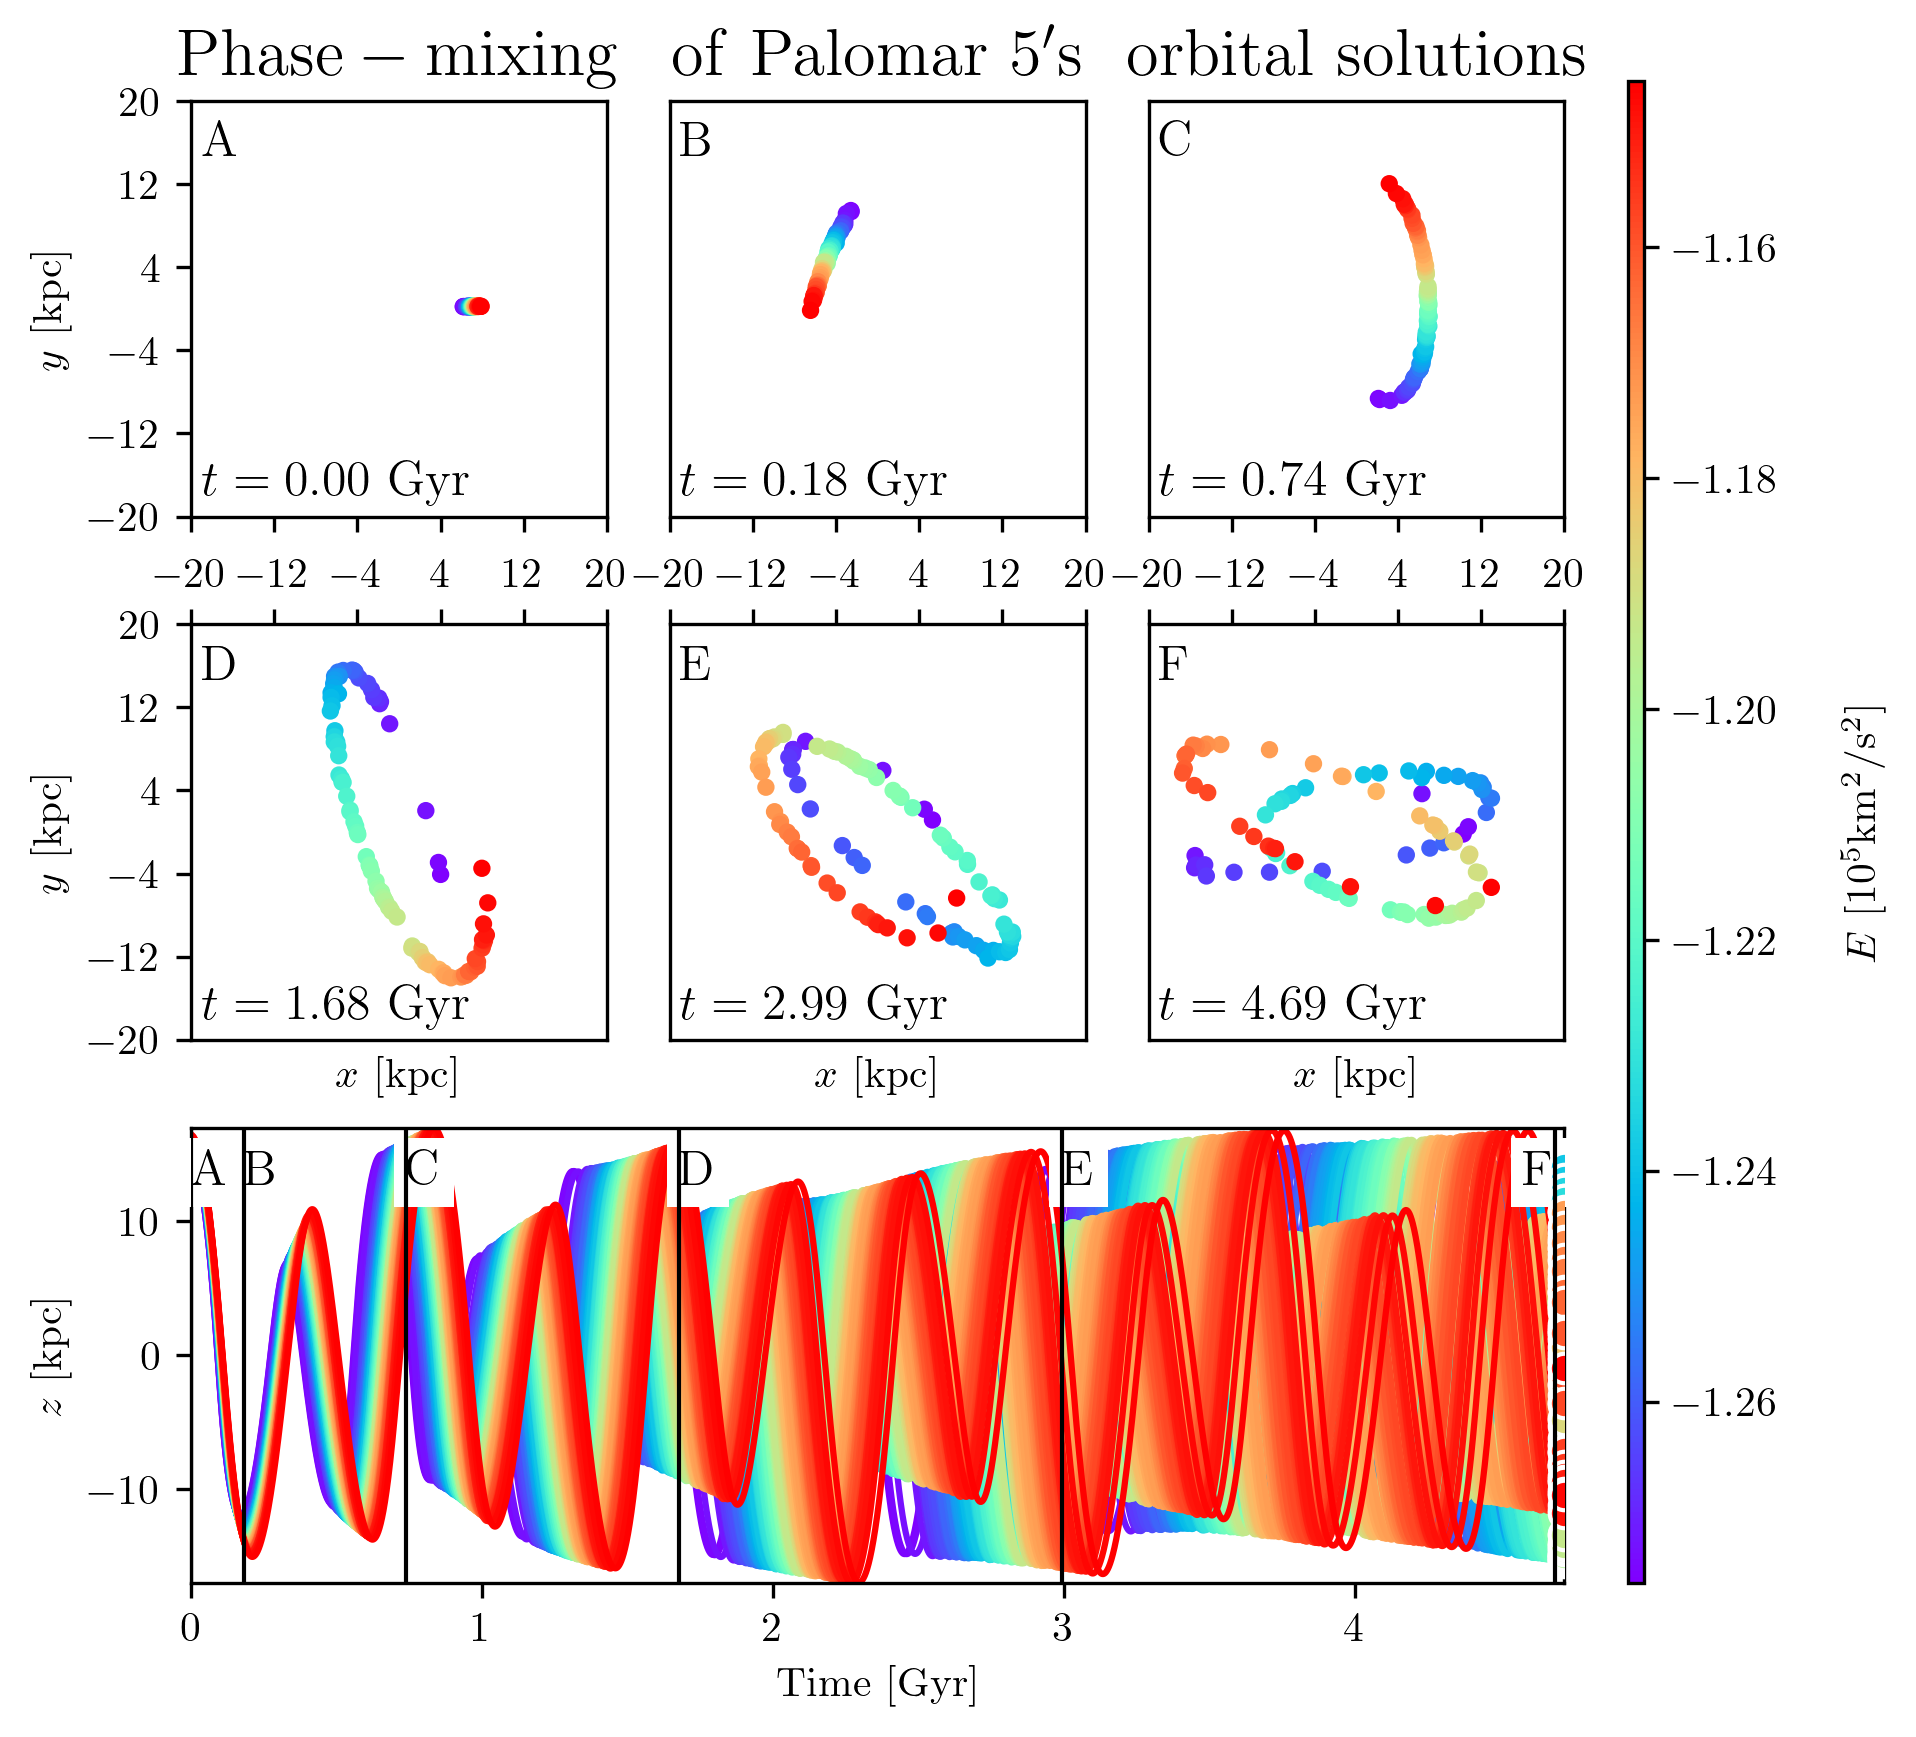
\includegraphics[width=\linewidth]{images/phase_mixing_palomar_5_orbital_solutions.png}
                \caption{Phase mixing of Palomar~5's orbital solutions in the \texttt{Pouliasis2017pii} potential. We sample 50 different initial conditions based on the observational uncertainties in distance, radial velocity, and proper motions. Each orbital solution is color-coded by its initial total orbital energy $E$. The top six panels show snapshots of the positions in the $xy$-plane of the orbital solutions at different times. The bottom panel shows the evolution of the $z$ coordinate as a function of time. Black vertical bars mark the timestamps corresponding to the snapshots in the top panels, which are labeled with matching alphabetical identifiers.}
                \label{fig:phase_mixing_palomar_5_orbital_solutions}
            \end{figure}    

            By inspecting Eq.\ref{EQ:phase_mixing}, we note that if the phase-mixing time is normalized by the characteristic orbital time, the resulting dimensionless mixing time is inversely proportional to the uncertainty in orbital energy. This relationship is general and holds for all orbits, regardless of their periods. However, it is still illustrative to examine this behavior in the context of the globular cluster catalog. In Fig.\ref{fig:phase_mixing_orbital_errors_sample}, I present the phase-mixing times for all Galactic globular clusters, based on current uncertainties from the Gaia DR3 catalog. The top panel shows the distribution for all 165 clusters. The bottom panels highlight the mixing behavior in cylindrical radius for a selection of statistically representative clusters: Gran~1, which has the shortest mixing time; Gran~5, the median case; NGC~6752, whose mixing time is closest to the mean; and NGC~2419, which has the longest mixing time.

            It is important to emphasize that these estimates are highly model-dependent. In some cases, the models predict phase-mixing timescales exceeding the age of the Universe. Unsurprisingly, the phase-mixing time correlates with the orbital period, which itself is related to the cluster's distance from the Galactic center. At large Galactocentric distances, the gravitational potential of the Milky Way becomes increasingly uncertain, as observational constraints on the Galactic mass distribution are weaker. Therefore, these extreme mixing times should not be interpreted as implying that we can predict the phase-space location of certain clusters with high confidence over cosmological timescales. 



            \begin{figure}
                \centering
                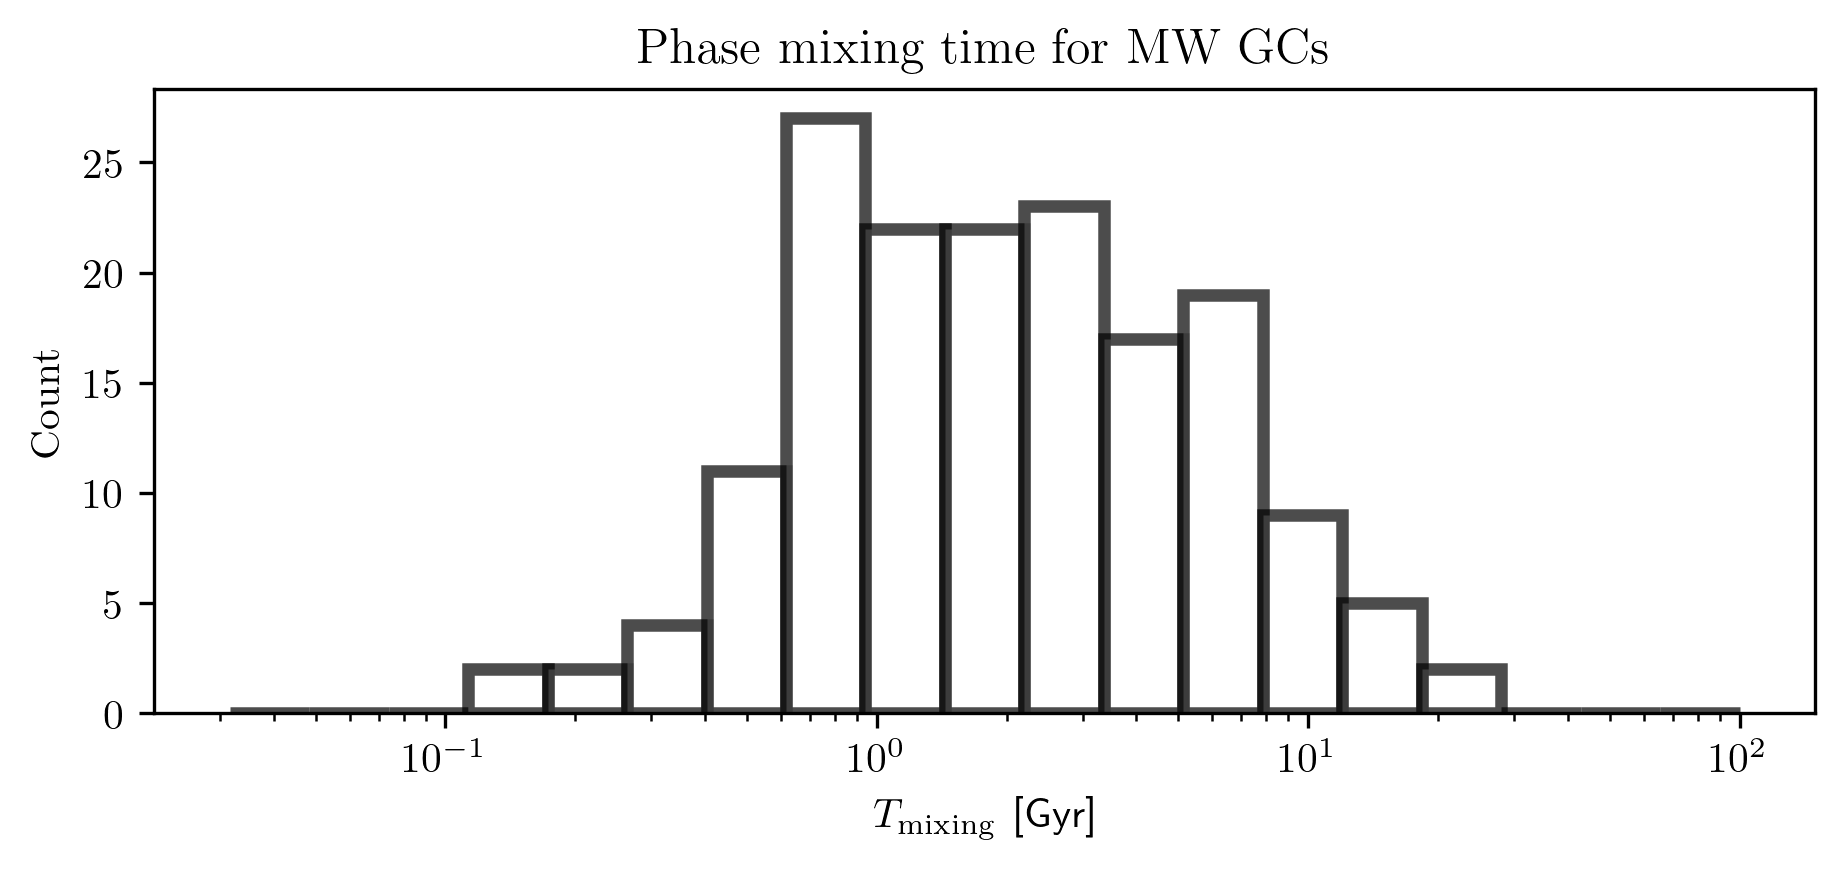
\includegraphics[width=.75\linewidth]{images/phase_mixing_time_histogram_MWGCS.png}
                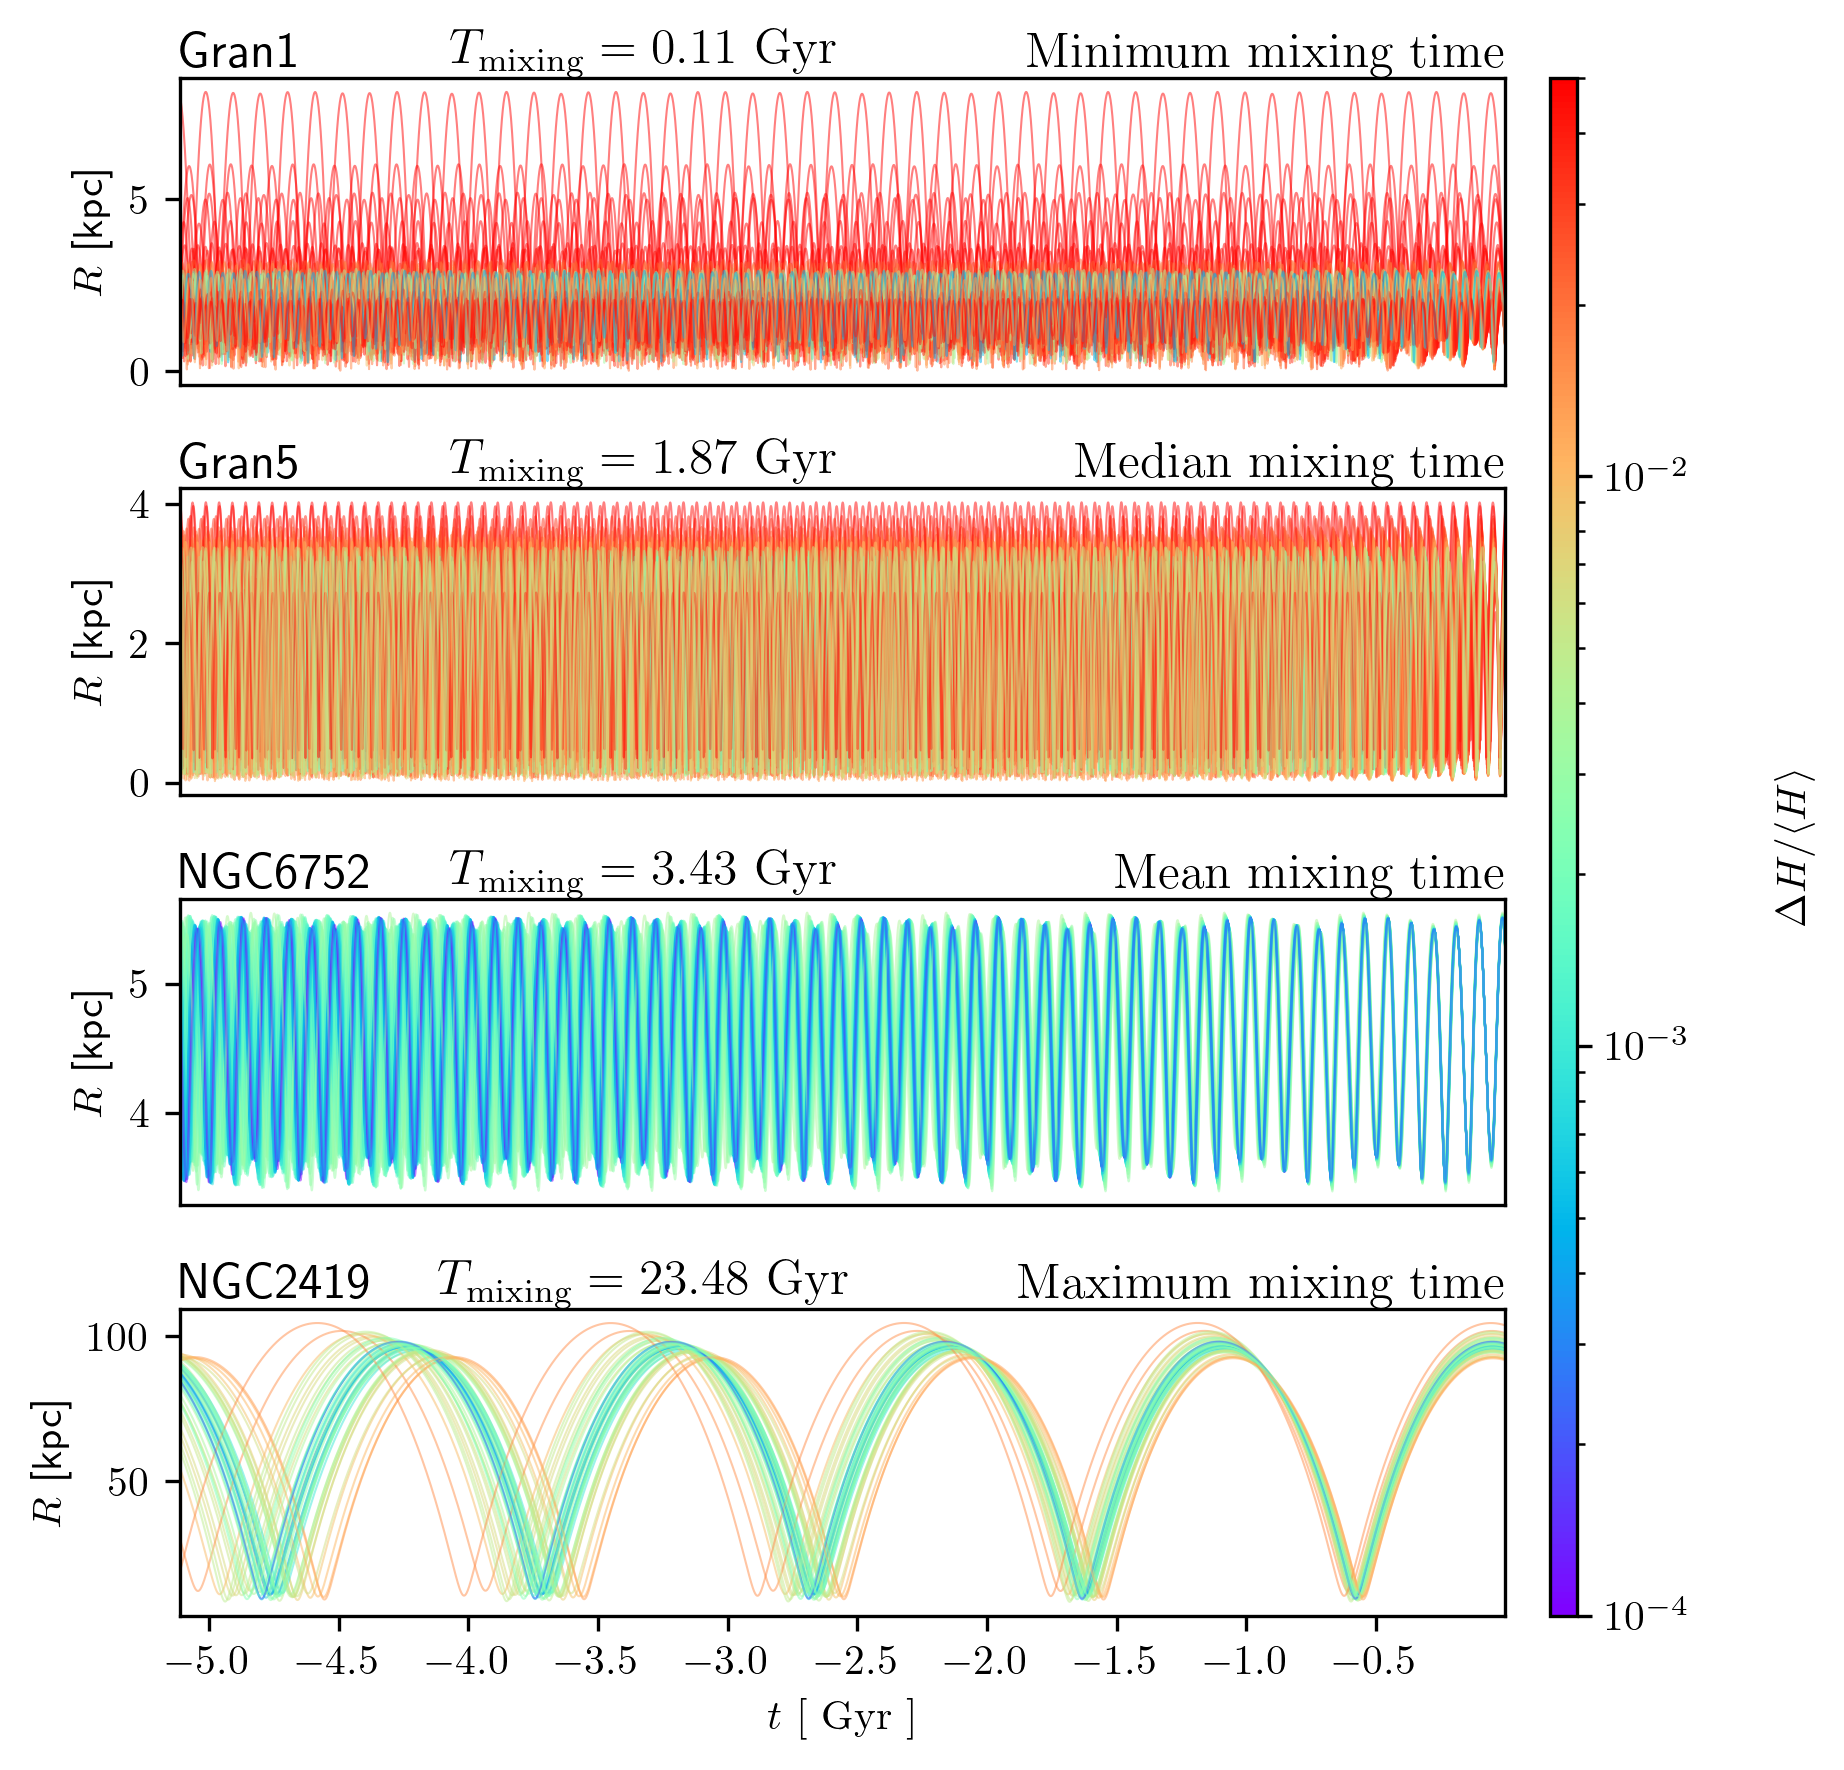
\includegraphics[width=\linewidth]{images/phase_mixing_orbital_errors_sample.png}
                \caption{The top panel shows the distribution of phase-mixing times for globular clusters, computed using Eq.~\ref{EQ:phase_mixing}. The following four rows illustrate the phase-mixing behavior for four selected clusters over the time range considered in this experiment. Orbital solutions are color-coded by their normalized deviation from the mean orbital energy.}
                \label{fig:phase_mixing_orbital_errors_sample}
            \end{figure}
     
            It's also interesting to note how the uncertainties in the orbital energy relates to the uncertainties in each observable. In Fig.~\ref{fig:energy_sensitivity_analysis_MWGCS_to_distance_RV_mu}, I perform this quick calulation. The uncertainties are measured in Galactic coordinates the ICRS coordinate system. This is a direct transformation to Galactic coordinates and thus can be expressed analytically.

            \begin{figure}[p]
                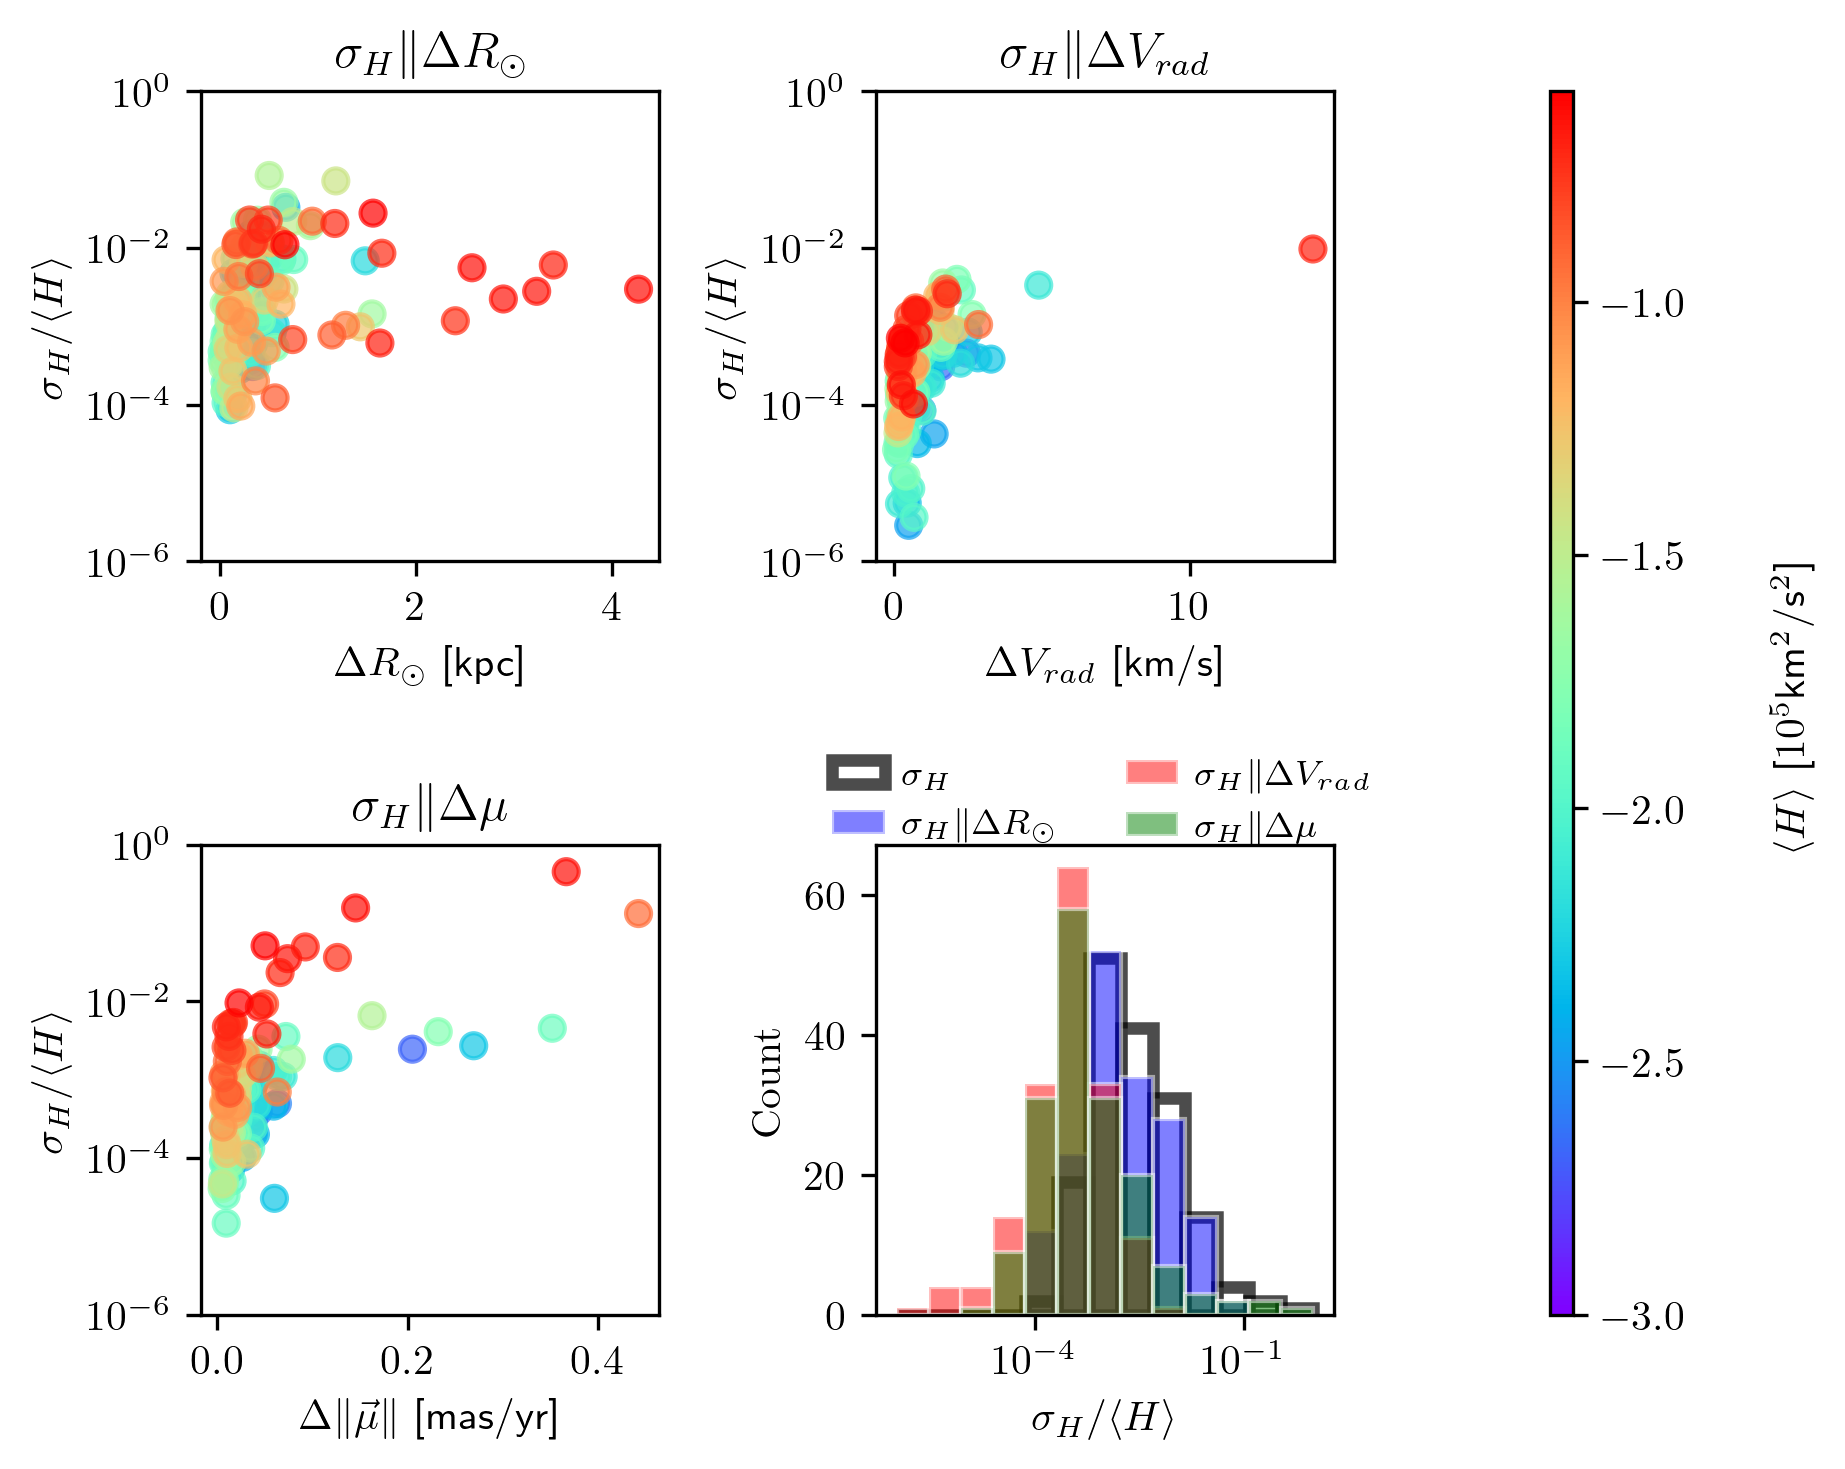
\includegraphics[width=\linewidth]{images/energy_sensitivity_analysis_MWGCS_to_errors.png}
                \caption{An analysis on the spread in orbital energies of the globular cluster population for each of its reported uncertainties. Each panel finds the STD in the Hamiltonain given the uncertainties in the specific variable. So the top left allows the distances to vary but holds the proper motions and radial velocities constant. It is plotted against the distance. The clusters are color-coated by their mean energies.}
                \label{fig:energy_sensitivity_analysis_MWGCS_to_distance_RV_mu}
            \end{figure}

        \subsubsection{Mixing of tidal debris}
            At first glance, Fig.~\ref{fig:phase_mixing_palomar_5_orbital_solutions} might give the impression that we are looking at snapshots of a single stellar stream at different times. In reality, the figure shows different orbital solutions. This visual similarity underscores that both phenomena—stellar streams and diverging orbital solutions—are manifestations of phase mixing. However, there is a crucial distinction: phase mixing of tidal debris is a physical process involving actual particles with slightly different initial conditions, whereas diverging orbital solutions represent the increasing uncertainty in predicted trajectories over time.

            Still, it is useful to use phase mixing as an analogy, though the physical assumptions differ. In particular, the analogy breaks down because globular clusters are self-gravitating systems: stars interact gravitationally and remain bound for a significant time. This self-gravity slows down the mixing process. The time it takes for a globular cluster to dissolve and distribute its stars uniformly in phase space is typically longer than the idealized mixing time given by Eq.~\ref{EQ:phase_mixing}.

            Let us briefly illustrate this with a conceptual calculation:

            \begin{itemize}
                \item \textbf{Case 1}: Particles drift apart under phase mixing with no mutual gravitational influence.
                \item \textbf{Case 2}: Particles are bound by a central potential, representing the cluster's self-gravity.
            \end{itemize}
            From this thought experiment, we see that phase mixing proceeds more slowly when self-gravity is included. Nevertheless, phase mixing still governs the long-term behavior of tidally escaped stars.

            Importantly, we need not consider all particles within the cluster to study phase mixing. For clusters with short orbital mixing times compared to the simulation duration, stars that escape during the simulation can redistribute throughout the available phase space. While the resulting debris will not be uniformly distributed—an overdensity will remain at the cluster location—the tidal debris will broadly fill the phase space accessible to it. This point is crucial for the results discussed in Chapter 4.




\section{The Ignored Physics}
    \subsection{Collisional dynamics}
        \begin{itemize}
            \item not nbody
            \item no mass segregation
            \item no three body encounters 
            \item no soft or hard binaries 
            \item show some results from Corespray 
        \end{itemize}
    
    \subsection{Stellar evolution}
        \begin{itemize}
            \item They're all point masses 
            \item No salpeter's 
            \item No strong initial mass loss 
            \item No accurate model for the colors 
            \item No multiple stellar populations 
        \end{itemize}
    
    \subsection{Time evolution}
        In someways, we take time evolution into account, and in someways, we ignore and this has already been covered in the previous sections. i.e., the orbit of the star-particles depend on the position of the host globular cluster, which I do not solve for simoltaneously but instead opt to load it into the computation, as shown in Section~\ref{subsec:myEquationsOfMotion}. Also, things like mass segregation and stellar evolution are time-dependent which is completely ignored in my simulations. 

